% !TEX root=../master.tex

\chapter[Error-State LQR Control of a Multirotor UAV]{Error-State LQR Control of a Multirotor UAV\protect\footnotemark}
\footnotetext{This chapter is a
modified version of the paper published in the 2019 International Conference on
Unmanned Aircraft Systems, written by Michael Farrell, James Jackson, Jerel
Nielsen, Craig Bidstrup, and Tim McLain~\cite{farrell2019error}. The coauthors
assisted with the mathematical notation and trajectory generation sections of
this paper.}
\label{chp:control_paper}

\graphicspath{{lqr_paper/}}

\section{Introduction}
% !TEX root=../root.tex

%\subsection{Background}

Over the past two decades, multirotor unmanned air vehicles (UAVs) have become a
popular platform for robotics research and the base for a variety of consumer and
commercial products. UAVs are currently used all over the world for everything
from military surveillance to package delivery. Larger multirotor vehicles
have even been recently introduced to transport humans. Whatever the
application, multirotors must but able to safely navigate in their environment,
requiring a combination of complex perception, motion planning, and control
algorithms. This paper describes a novel control algorithm that allows a multirotor UAV to
accurately track a desired trajectory in time and space. 

% - UAV control
% - Lie Algebra in estimation Geometric Control
% - Duality to ESKF
% !TEX root=../root.tex

%\subsection{Related Works}

The Linear Quadratic Regulator (LQR) is a well-known feedback controller that
computes the optimal feedback gains for a linear time-invariant (LTI) system
given a quadratic cost function. LQR has been used to control multirotor UAVs with a variety of
approaches. Almost all of these approaches
linearize the system at a given stable state and use a fixed LQR
gain~\cite{cowling2007prototype}. Some have
used a gain scheduling approach with a library of LQR gains for different
magnitudes of deviation from the desired state~\cite{reyes2013lqr}. Recently, an approach was
proposed that relinearizes the system at a fixed rate, slower than the control
loop, and then recomputes the LQR gains at that rate~\cite{foehn2018onboard}. Our
proposed solution takes a similar approach while relinearizing and recomputing
the LQR gains at every control step. 

Recently there has been a movement in the robotics community to appropriately
deal with the evolution of a robot's state along a manifold using Lie
theory~\cite{sola2018micro}. Though these methods have widely been used in the
field of state estimation~\cite{sola2017quaternion,koch2017relative}, a
% field of state estimation~\cite{sola2017quaternion}~\cite{koch2017relative}, a
few methods have emerged that also apply Lie theory to
control~\cite{yu2015high,lee2010geometric}. We propose a formulation of
% control~\cite{yu2015high}~\cite{lee2010geometric}. We propose a formulation of
the LQR problem that properly deals with the manifold nature of the state,
specifically the attitude component. Most previous LQR solutions
for a multirotor UAV use an Euler angle representation of attitude and treat the
tuple of ZYX Euler angles as if it were a vector space~\cite{cowling2007prototype}, even
though it is not~\cite{diebel2006representing}. While some methods use unit
quaternions or rotation matrices to properly represent atttiude, these are also
not inherently a vector space and extra steps are required to orthonormalize or
otherwise force the attitude to stay on the
manifold~\cite{reyes2013lqr,foehn2018onboard}. The proposed solution is
derived from Lie theory and care is taken to ensure that all vector
manipulations are done with
appropriate vector quantities so that the state remains on the manifold.

% \begin{figure}
  % \centering
  % 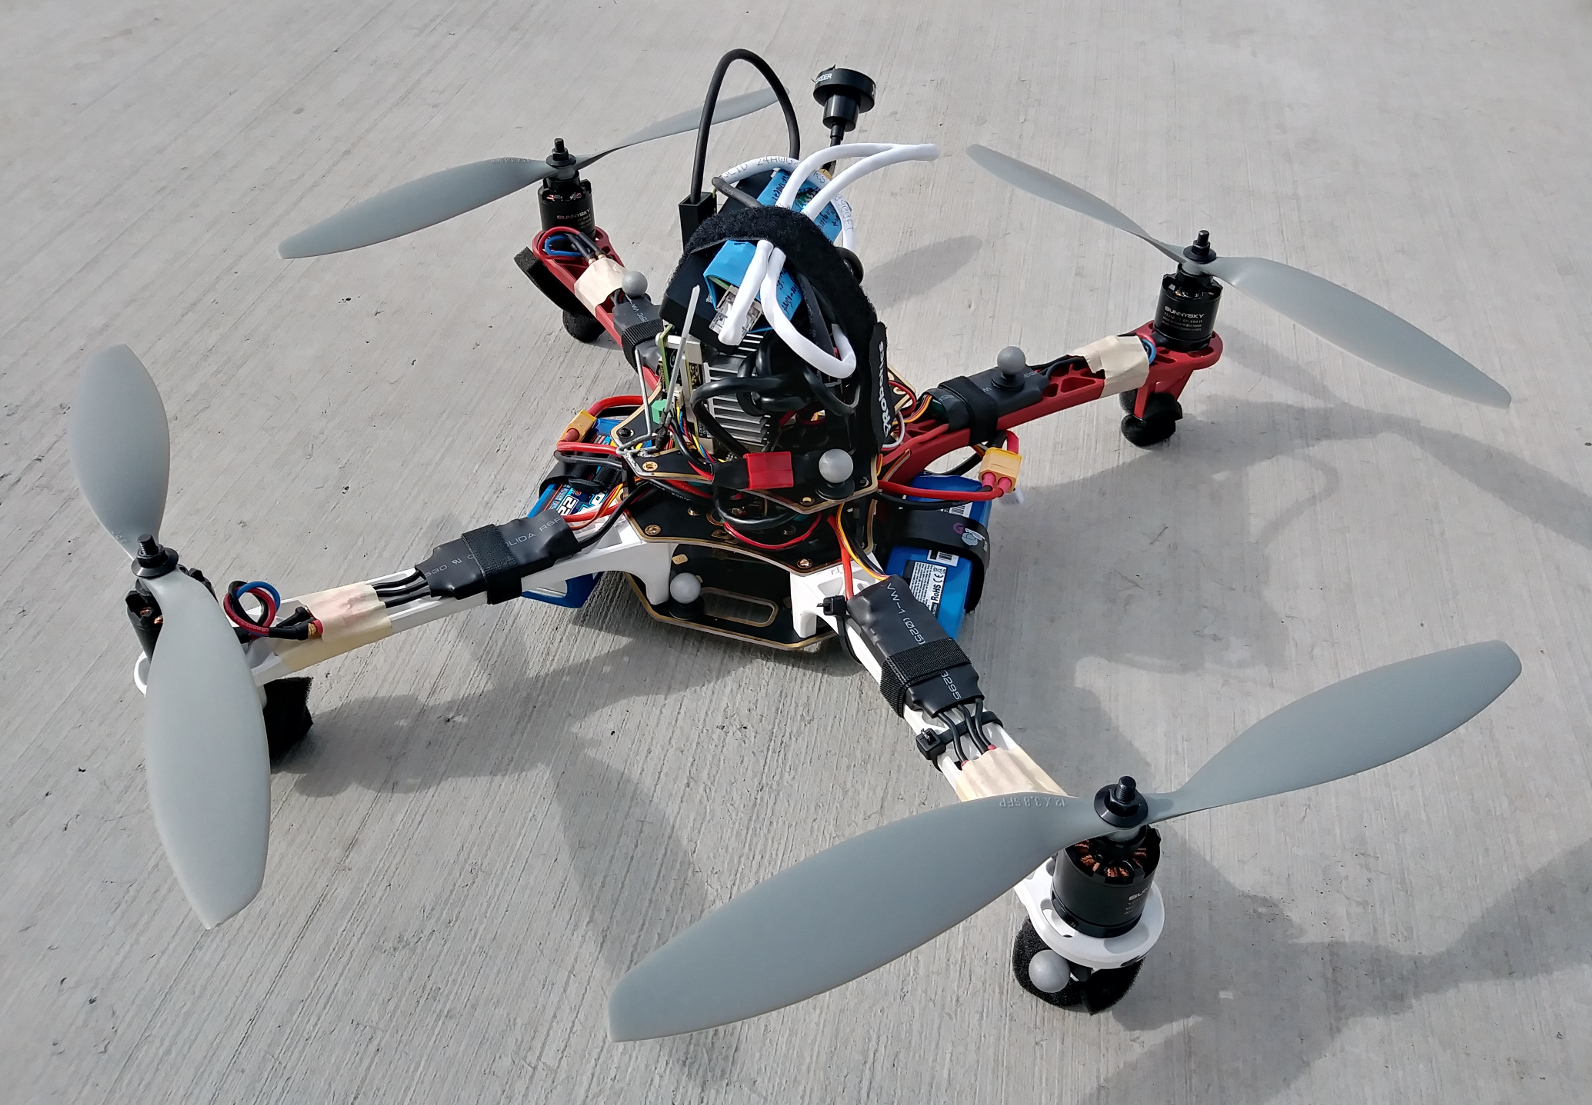
\includegraphics[scale=0.15]{figures/hardware_platform.jpg}
  % \caption[Multirotor UAV Used in Experiments]{Hardware platform used in experiments.}
  % \label{f:drone_pic}
% \end{figure}

% !TEX root=../root.tex

%\subsection{Paper Layout}

\secref{sec:model} explains the multirotor UAV model used in the proposed
controller formulation. \secref{sec:lqr_control} presents traditional LQR
theory and shows how the proposed LQR formulation is a natural extension when
care is taken to apply Lie theory to the multirotor problem.
\secref{sec:experiment} describes the experiments used to demonstrate the
proposed control scheme both in simulation and in hardware.
\secref{sec:results} discusses the results of the experiments and
\secref{sec:conclusion} provides concluding remarks.


\section{Model} \label{sec:model}
% !TEX root=../root.tex

\subsection{Notation}

We define some common notation used throughout the paper, first noting that
vectors are represented with a bold letter (e.g., $\bf v$) and matrices with a
capital letter (e.g., $A$).
\begin{center}
\begin{tabularx}{\columnwidth}{lX}
$R_a^b$ & Rotation matrix from reference frame $a$ to $b$ \\
$\vect{v}_{a/b}^c$ & Vector state $\vect{v}$ of frame $a$ w.r.t.~frame $b$, expressed in frame $c$ \\
% $\hat{a}$ & Estimate of true variable $a$ \\
% $\bar{a}$ & Measurement of $a$ \\
$\des{a}$ & Desired value of $a$ \\
$\dot{a}$ & Time derivative of $a$ \\
$\tilde{a}$ & Error of variable $a$, i.e., $\tilde{a} \triangleq a - \des{a}$
\end{tabularx}
\end{center}
%
We also define the following coordinate frames:
\begin{center}
\begin{tabularx}{\columnwidth}{lX}
$I$ & The inertial coordinate frame in north-east-down\\
$\ell$ & The aircraft's vehicle-1 (body-level) coordinate frame \\
$b$ & The aircraft's body-fixed coordinate frame
\end{tabularx}
\end{center}

We make frequent use of the skew-symmetric matrix operator defined by
\begin{equation}
  \skewmat{\vect{v}} \triangleq
  \begin{bmatrix}
  0 & -v_{3} & v_{2}\\
  v_{3} & 0 & -v_{1}\\
  -v_{2} & v_{1} & 0
  \end{bmatrix},
\end{equation}
which is related to the cross-product between two vectors as
\begin{equation}
  \vect{v}\times\vect{w}=\skewmat{\vect{v}}\vect{w}.
\end{equation}
We also use the standard basis vectors $\vect{e}_1, \vect{e}_2, \ldots, \vect{e}_N$, where $\vect{e}_1 = \begin{bmatrix} 1 & 0 & \cdots & 0 \end{bmatrix}^\transpose$ and so forth.

% !TEX root=../root.tex

\subsection{Quaternion Representation}
\label{appx:quaternions}
A quaternion $\q$ is a hyper-complex number of rank four.  It is well known that
a unit quaternion $\in S^3$ can be used to efficiently represent attitude, as
$S^3$ is a double cover of $\SO(3)$.  Quaternions have the advantage over
$\SO(3)$ of being more efficient to implement on modern hardware~\cite{casey2013AttitudeRepresentation}, therefore in the software implementation of the described algorithm, we use quaternions, rather than rotation matrices.

We use Hamiltonian notation for unit quaternions $\in S^3$
\begin{equation}
\q=\begin{pmatrix}q_{0} & q_{x}i & q_{y} j & q_{z}k \end{pmatrix}%=\begin{pmatrix}q_{0} & \bar{\q} \end{pmatrix},
\end{equation}
and define the complex numbers $i$, $j$, and $k$, such that
\begin{equation}
\begin{array}{rrrcc}
	& & ij &= -ji &= k, \\
	& & jk &= -kj &= i, \\
	& & ki &= -ik &= j, \\
	i^2 &= j^2 &= k^2 & = ijk &= -1.
\end{array}
\end{equation}
For convenience, we sometimes refer to the complex portion of the quaternion as
\begin{equation}
	\bar{\q} = \begin{bmatrix} q_x & q_y & q_z \end{bmatrix} ^\transpose
\end{equation}
and write quaternions as the tuple of the real and complex portions
\begin{equation}
	\q = \begin{pmatrix} q_0 \\ \bar{\q} \end{pmatrix}.
\end{equation}

Given our use of the Hamiltonian notation, the quaternion group operator
$\otimes$ can be written as the following matrix-like product
\begin{equation}
	\q^a \otimes \q^b = \begin{pmatrix} -q_0^a & \left(-\bar{\q}^{a}\right)^\transpose \\ \bar{\q}^a & q^a_0 I + \skewmat{\bar{\q}^a} \end{pmatrix}
	\begin{pmatrix} q^b \\ \bar{\q}^b\end{pmatrix}.
\end{equation}
It is often convenient to convert a quaternion $\q$ to its associated passive rotation matrix.  This is done with
\begin{equation}
\label{eq:R_from_q}
R\left(\q\right)=\left(2q_{0}^{2}-1\right)I-2q_{0}\skewmat{\bar{\q}}+2\bar{\q}\bar{\q}^{\top}\in SO\left(3\right).
\end{equation}

We also need to frequently convert between the Lie group, $S^3$, and the Lie
algebra, $\mathbb{R}^3$, which enables us to operate in a vector space. This is done with the
exponential and logarithmic mappings. The exponential mapping for a unit quaternion is defined as
\begin{align}
\exp_{\q} & :\mathbb{R}^{3}\rightarrow S^3\nonumber \\
\exp_{\q}\left(\vect{\delta}\right) & \triangleq\begin{bmatrix}\cos\left(\frac{\lVert\vect{\delta}\rVert}{2}\right)\\
\sin\left(\frac{\lVert\vect{\delta}\rVert}{2}\right)\frac{\vect{\delta}}{\lVert\vect{\delta}\rVert}
\end{bmatrix},\label{eqn:exponential_map}
\end{align}
with the corresponding logarithmic map defined as
\begin{align}
\log_{\q} & :S^3\rightarrow \mathbb{R}^{3}\nonumber \\
\log_{\q}\left(\q\right) & \triangleq2\;\mathrm{atan2}\left(\left\Vert \bar{\q}\right\Vert ,q_{0}\right)\frac{\bar{\q}}{\left\Vert \bar{\q}\right\Vert }.\label{eqn:log_map}
\end{align}
To avoid numerical issues when $\norm{\vect{\delta}}\approx0$, we also employ the small-angle approximations of the quaternion exponential and logarithm
\begin{align}
\exp_{\q}\left(\vect{\delta}\right) & \approx\begin{bmatrix}1\\
\frac{\vect{\delta}}{2}
\end{bmatrix}\label{eq:quaternion_exp_approx}\\
\log_{\q}\left(\q\right) & \approx2\;\textrm{sign}\left(q_{0}\right)\bar{\q}.\label{eq:quaternion_log_approx}
\end{align}

We also note that rotations may be written equivalently as $\q_a^b=R\left(\q_a^b\right)=R_a^b$, where the choice of these is dictated by convenience.
We use passive rotation matrices, meaning that the rotation matrix $R_a^b$ acts
on a vector $\vect{r}^a$, expressed in frame $a$, and results in the same
vector, now expressed in frame $b$ as
\begin{equation}
\vect{r}^b = R_a^b \vect{r}^a .
\end{equation}

% The $\boxplus$/$\boxminus$ notation for unit quaternions is now defined by
% \begin{align*}
% \boxplus: & S^3\times\mathbb{R}^{3}\rightarrow S^3\\
%  & \q\boxplus\vect{\delta}\triangleq\q\otimes\exp_q\left(\vect{\delta}\right)\\
% \boxminus: & S^3\times S^3\rightarrow\mathbb{R}^{3}\\
%  & \q\boxminus\vect{p}\triangleq\log_q\left(\vect{p}^{-1}\otimes\q\right).
% \end{align*}
% Let's look at one application for clarification.
% With body angular rate $\vect{\omega}_{b/i}^b$, inertial to body rotation $\q_i^b$, and $\vect{\theta}=\vect{\omega}_{b/i}^b \Delta t$, we have
% \begin{align}
% \q_i^b\left(t+\Delta t\right) & =\q_i^b\left(t\right)\boxplus\vect{\theta}\\
% \vect{\theta} & =\q_i^b\left(t+\Delta t\right)\boxminus\q_i^b\left(t\right).
% \end{align}

%\subsection{Quadrotor Dynamics With Quaternion Attitude}
%In the associated software library, we employ the following dynamics for the quadrotor:
%\begin{align}
    %\dot{\vect{p}}_{b/I}^{I} &= 	R\left(\q_{I}^{b}\right)^\transpose \vect{v}_{b/I}^{b} \nonumber \\
	%\dot{\q}_{I}^{b} &= - \frac{1}{2} \begin{pmatrix} 0 \\ \omega_{b/I}^b\end{pmatrix} \otimes \q_I^b\nonumber\\
	%\dot{\vect{v}}_{b/I}^{b} 
	%&= 	g\frac{s}{s_e}\vect{e}_3 + gR\left(\q_I^b\right) \vect{e}_3- \drag\vect{v}_{b/I}^b - \skewmat{\vect{\omega}_{b/I}^b}\vect{v}_{b/I}^b.
	%\label{eq:quat_dynamics}
%\end{align}
%and we solve this using a fourth-order Runge-Kutta extension of \eqref{eq:quaternion_integration}.

% TODO maybe pull from here
%\subsection{Quaternion Error State Dynamics}
%As with the rotation matrix, we wish to find a minimal representation of the error about a quaternion attitude state.  Let us start with the differential equation for quaternion dynamics
%\begin{equation}
	%\dot{\q}_{I}^{b} = \frac{1}{2}\q_I^b \otimes \begin{pmatrix} 0 \\ \vect{\omega}_{b/I}^b\end{pmatrix}.
%\end{equation}
%This can be solved using the quaternion exponential with
%\begin{equation}
	%\q_I^b\left(t\right) = \q_I^b\left(0\right)\otimes\exp_{\q}\left(\int_0^t \vect{\omega}_{b/I}^b\left(\tau\right) d\tau \right).
%\end{equation}
%To reduce this to our minimal vector representation, as we did with rotation matrices in \eqref{eq:att_vector}, let us define the attitude vector $\vect{r}_I^b\left(t\right)=\vect{r}_I^b\left(t_0\right)+\int_{t_0}^t\boldsymbol{\omega}_{b/I}^b\left(\tau\right)d\tau$ with $\vect{r}_I^b\left(t_0\right)=0$ such that
%\begin{equation}
	%\q_I^b\left(t\right) = \q_I^b\left(0\right)\otimes\exp_{\q}\left(\vect{r}_I^b\left(t\right) \right).
%\end{equation}
%It then follows that the error state of our attitude vector is
%\begin{align}
	%\tilde{\vect{r}}_I^{b} 
		%&= \vect{r}_I^b - \hat{\vect{r}}_I^{\hat{b}}  \nonumber \\
		%&= \vect{r}_I^b - R\left(\q_I^b\right) R\left(\q_I^{\hat{b}}\right)^\transpose \hat{\vect{r}}_I^{\hat{b}}\nonumber \\
		%&= \vect{r}_I^b - R\left(\tilde{\q}_{\hat{b}}^b\right)  \hat{\vect{r}}_I^{\hat{b}}
%\end{align}
%and its time derivative is
%\begin{equation}
	%\dot{\tilde{\vect{r}}}_I^{b} = \dot{\vect{r}}_I^b - R\left(\tilde{\q}_{\hat{b}}^b\right)  \dot{\hat{\vect{r}}}_I^{\hat{b}}.
%\end{equation}
%\subsection{Quaternion Trajectory Generation}
%When creating trajectories using differential flatness for quaternion attitude states, the equivalent expression to \eqref{eq:des_attitude} is
%\begin{equation}
	%\des{q}_I^b = \exp_{\q}\left(\vect{e}_3\des{\psi}_{b/I}^I)\right) \otimes \exp_{\q}\left(\theta \vect{\delta}\right) \label{eq:des_attitude}
%\end{equation}
%where, as in \eqref{eq:des_attitude}, $\theta\vect{\delta}$ is the axis-angle error between the desired acceleration and the inertial z-axis.

%% !TEX root=../root.tex

\subsection{Rotations}
\MF{If we use quaternions throughout (because thats part of the point) maybe we
don't need this. But we can take the first talk about passive rotations}

We use passive rotation matrices, meaning that the rotation matrix $R_a^b$ acts on a vector $\vect{r}^a$, expressed in frame $a$, to express it in frame $b$ as
\begin{equation}
\vect{r}^b = R_a^b \vect{r}^a .
\end{equation}
By representing orientation states directly as rotation matrices, as opposed to other representations such as Euler angles or axis-angle, the group structure of the rotation is preserved.
While unit-quaternions also preserve the group structure in a more concise representation, we choose rotation matrices for clarity of presentation in the following derivations.
However, the companion software library implements techniques described in this paper using quaternions, and the mapping between the rotation-matrix and quaternion representations is described in \appxref{appx:quaternions}.

Rotation matrices are elements of the special orthogonal group $\SO(3)$, where the group operator is matrix multiplication.
Incremental changes or perturbations happen in the tangent space.
The tangent space at the identity element $R=I$ is the Lie algebra $\so(3)$.
The exponential and logarithmic mappings map between the group and the algebra:
\begin{align}
\exp &: \so(3) \to \SO(3) \\
\log &: \SO(3) \to \so(3)
\end{align}
For $\SO(3)$ these mappings are the matrix exponential and matrix logarithm.

The Lie algebra is a vector space, and so is isomorphic to $\mathbb{R}^3$.
The hat $^\wedge$ and vee $^\vee$ operators describe this invertible mapping:
\begin{align}
^\wedge &: \mathbb{R}^3 \to \so(3) \\
^\vee &: \so(3) \to \mathbb{R}^3 .
\end{align}
For $\so(3)$ the $^\wedge$ operator is the skew-symmetric operator:
\begin{equation}
^\wedge : \vect{v} \mapsto \skewmat{\vect{v}} ,
\end{equation}
and the $^\vee$ operator is simply the inverse operation.

For convenience in writing differential quantities as vectors in $\mathbb{R}^3$, we define the capitalized exponential and logarithmic mappings as
\begin{align}
\Exp &: \mathbb{R}^3 \to \SO(3) \\
\Exp &: \vect{\omega} \mapsto \exp(\vect{\omega}^\wedge) ,
\end{align}
and
\begin{align}
\Log &: \SO(3) \to \mathbb{R}^3 \\
\Log &: R \mapsto \log(R)^\vee .
\end{align}
For $\SO(3)$, a closed-form solution for the $\Exp$ mapping is given by the Rodriques formula.
These operators are related to the $\boxplus$/$\boxminus$ notation originally described in~\cite{hertzberg2013integrating} as
\begin{align}
R \boxplus \vect{\omega} &\triangleq R \Exp(\vect{\omega}) , \\
R_2 \boxminus R_1 &\triangleq \Log({R_1}^\transpose R_2) .
\end{align}
\DK{Do we want a symbol for the group operator? (e.g. $R_1 \circ R_2$ or $R_1 \cdot R_2$ vs $R_1 R_2$)}

% !TEX root=../root.tex

\subsection{Quadrotor Dynamics}

If we define the state of a quadrotor as the tuple of position, velocity, and
attitude
\begin{equation*}
	%\vect{x} = \begin{pmatrix}\vect{p}_{b/i}^{i}, R_{i}^{b},
        %\vect{v}_{b/i}^{b} \end{pmatrix} \in \mathbb{R}^3 \times \mathbb{R}^3
        %\times S^3
  \vect{x} = \begin{pmatrix}\vect{p}_{b/I}^{I}, \vect{v}_{b/I}^b, \vect{q}_I^{b}
        \end{pmatrix} \in \mathbb{R}^3 \times \mathbb{R}^3
        \times S^3
\end{equation*}
and the input to our system as the tuple of the throttle signal, $s$, and angular
velocity, $\vect{\omega}_{b/I}^b$,
\begin{equation*}
	\vect{u} = \begin{pmatrix}s, \vect{\omega}_{b/i}^b \end{pmatrix} \in
        \mathbb{R}^1 \times \mathbb{R}^3,
\end{equation*}
then the rigid body dynamics of a multirotor UAV are as follows~\cite{leishman2014accel}:
\small
\begin{align}
	% \dot{\vect{x}} &= f\left(\vect{x}, \vect{u}\right) \nonumber \\
	% \begin{pmatrix} 
		\dot{\vect{p}}_{b/I}^{I} &= \left(R_{I}^{b}\right)^\transpose \vect{v}_{b/I}^{b} \nonumber \\
		\dot{\vect{v}}_{b/I}^{b} &= gR_I^b \vect{e}_3 - g\frac{s}{s_e}\vect{e}_3 -
                \drag \left( I - \vect{e}_3 \vect{e}_3^\top \right)
                \vect{v}_{b/I}^b -
                \skewmat{\vect{\omega}_{b/I}^b}\vect{v}_{b/I}^b
                \label{eq:dynamics} \\
                \dot{\vect{q}}_{I}^{b} 
	% \end{pmatrix}
	&= 	
	% \begin{pmatrix} 
		% \left(R_{I}^{b}\right)^\transpose \vect{v}_{b/I}^{b} \\
		% gR_I^b \vect{e}_3 - g\frac{s}{s_e}\vect{e}_3 -
  %               \drag \left( I - \vect{e}_3 \vect{e}_3^\top \right) \vect{v}_{b/I}^b -
  %               \skewmat{\vect{\omega}_{b/I}^b}\vect{v}_{b/I}^b\\
		%-\skewmat{\vect{\omega}_{b/I}^b} R_{I}^{b}
                \q_I^b \otimes \begin{pmatrix} 0 \\ \frac{1}{2}
                \omega_{b/I}^b\end{pmatrix} \nonumber,
	% \end{pmatrix},
\end{align}
\normalsize
where $\drag$ is a linear drag constant, $s_e$ is the throttle command required to hover, and $g$ is the magnitude of gravity.  This model assumes a linear relationship between throttle signal and thrust, which is not always the case.  Although we use this simple model, more sophisticated approaches, such as~\cite{small2018mpc} estimate this relationship online and compensate for it in real time.

%While the differential equation given in~\eqref{eq:dynamics} can be solved in a number of ways, it is important to properly account for
%the manifold nature of the quaternion attitude representation, otherwise the
%integrated attitude will depart from $S^3$.
%and an expensive re-orthonormalization step will be required to ensure the rotation matrix remains member of $\SO(3)$.  A basic zero-order hold integration scheme is given in Appx.~\ref{appx:manifold_integration} where the attitude is integrated on the manifold and a more accurate fourth-order Runga-Kutta method on the manifold is used in the accompanying software library.

\subsection{Error-State Dynamics} \label{subsec:error_state_dyn}

It is useful to consider what is known as the \emph{error state} of the
quadrotor.  This concept has a long history in state estimation and is used in
the error-state Kalman
filter~\cite{sola2017quaternion,Markley2004MultiplicativeVA}.  The error state
is used in state estimation as a principled way to represent the covariance
about attitude in terms of a vector space, as opposed to some local
approximation.  This relationship is also useful in control for the same reason.
Performing control in the vector space of error state provides a principled way
to leverage well-understood and efficient linear algebra machinery to solve
control problems over non-vector quantities, such as attitude.  

We define the error state of some quantity $\vect{y}$ as
\begin{equation}
  \tilde{\vect{y}}=\vect{y} \boxminus \des{\vect{y}},
  \label{eq:error}
\end{equation}
where $\boxminus$ is an appropriate difference operator, as described
by~\cite{hertzberg2013integrating}.  For instance, if $\vect{y}$, 
$\des{\vect{y}}$ $\in \mathbb{R}^{n}$, the $\boxminus$ operator may be
defined as the vector subtraction operator. However, due to the attitude component of our
state, the vector subtraction operator is not defined between $\x$ and
$\des{\x}$. We instead define the
error state piecewise for
each component of the state and combine these into an error-state vector
\begin{equation}
  \tilde{\vect{x}}=\begin{bmatrix}{\tilde{\vect{p}}}_{b/I}^{I} &
  \tilde{\vect{v}}_{b/I}^{b} &
\tilde{\vect{r}}_{I}^{b}\end{bmatrix}^{\top}\in\mathbb{R}^{9\times1},
  \label{eq:error_state}
\end{equation}
where $\tilde{\vect{p}}_{b/I}^{I}$ is the error state associated with
position, $\tilde{\vect{v}}_{b/I}^{b}$ is the error state associated with
velocity, and $\tilde{\vect{r}}_{I}^{b}$ is the error state associated
with attitude.
%While the state itself is a not a vector quantity due to the attitude
%representation, the error state \emph{is} a vector
%quantity, allowing us to use many common techniques to perform control.

In our case, the error states associated with
position and velocity are simply defined using vector subtraction
\begin{align}
  \label{eq:pos_err}
  \tilde{\vect{p}}_{b/I}^{I} &= \vect{p}_{b/I}^{I} - \des{\vect{p}}_{b/I}^{I} \\
  \tilde{\vect{v}}_{b/I}^{b} &= \vect{v}_{b/I}^{b} - \des{\vect{v}}_{b/I}^{b},
  \label{eq:vel_err}
\end{align}
however, the error state associated with attitude is more complicated.
%In simplest terms, the subtraction operator is
%not a sensible operation for a unit quaternion, therefore we must turn to other
%methods to define the error state.

It is commonly understood that any representation of attitude has three
underlying degrees of freedom.  A unit quaternion has four parameters, but its
error can be described in terms of three degrees of freedom that we wish
to represent as a vector quantity.   In a neighborhood sufficiently close to the
identity,
these behave similarly to the Euler angle representation of roll, pitch,
and yaw. However, Euler angles are not a vector because the sequential rotation
method used to define Euler angles nonlinearly couples the three degrees of
freedom. Therefore, we define the vector
\begin{equation}
  \label{eq:r_def}
  \vect{r}_I^b\left(t\right)=\vect{r}_I^b\left(t_0\right)+\int_{t_{0}}^{t}\vect{\omega}_{b/I}^{b}\left(\tau\right)d\tau,
\end{equation}
such that $\vect{r}_I^b\left(t_0\right) = 0$ and $\dot{\vect{r}}_I^b = \vect{\omega}_{b/I}^{b}$.
With this definition, we can use~\eqref{eqn:exponential_map}
and~\eqref{eqn:log_map} to express
\begin{align}
  \label{eq:q_des}
  \q_{I}^{b} &= \des{\q}_{I}^{b} \otimes \exp_{\q} \left(\tilde{\vect{r}}\right) \\
  \tilde{\vect{r}} &= \log_{\q} \left(\left(\des{\q}_{I}^{b}\right)^{-1} \otimes
    \q_{I}^{b}\right),
\end{align}
as described by~\cite{hertzberg2013integrating}.

Even though $\vect{r}_I^b$ is a vector, we cannot simply compute the error state
as $\tilde{\vect{r}}_I^b=\vect{r}_I^b-\des{\vect{r}}_I^b$ because $\vect{r}_I^b$
is a minimal representation of $\vect{q}_I^b$, which is a double cover of the
Lie group $\SO\mathopen{}\mathclose\bgroup\left(3\aftergroup\egroup\right)$. %$SO\left(3\right)$.
Vector subtraction of members in this group is not valid.
However, the derivative of $\vect{r}_I^b$ exists in the tangent space of $\SO\mathopen{}\mathclose\bgroup\left(3\aftergroup\egroup\right)$, so we can perform
\begin{equation}
\label{eq:rdot_diff}
\dot{\tilde{\vect{r}}}_I^b=\dot{\vect{r}}_I^b-R_I^b\left(\des{R}_I^b\right)^{\top}\dot{\des{\vect{r}}}_I^b,
\end{equation}
where $R_I^b\left(\des{R}_I^b\right)^{\top}$ moves the desired vector
derivative, $\dot{\des{\vect{r}}}_I^b$, from its own tangent space to the tangent space of $\dot{\vect{r}}_I^b$.
With both vectors in the same tangent space, the vector subtraction in~\eqref{eq:rdot_diff} is valid.

For use in control, we similarly define an error state for the control input
with the error state being the difference between the current control input and
some reference input.
Using the same definition as in~\eqref{eq:error}, we can see that
\begin{align}
  \tilde{s} &= s - \des{s} \\
  \tilde{\vect{\omega}}_{b/I}^{b} &= \vect{\omega}_{b/I}^{b} - \des{\vect{\omega}}_{b/I}^{b}
  \label{eq:input_error_state}
\end{align}
where $\des{s}$ and $\des{\vect{\omega}}_{b/I}^{b}$ are respectively the reference throttle
signal and reference angular velocity. Note that we do not model the dynamic
response to these inputs. Instead, our model assumes that the multirotor
instantaneously reaches any commanded throttle and angular velocity.

Using the error-state definitions above, we can derive the error-state dynamics
of the quadrotor as
%\begin{equation}
	%\begin{pmatrix} 
                %\dot{\tilde{\vect{p}}}_{b/I}^{I}\\ 
                %\dot{\tilde{\vect{v}}}_{b/I}^{b}\\
                %\dot{\tilde{\vect{q}}}_{I}^{b} 
	%\end{pmatrix}
	%= 	
        %\begin{pmatrix} \left(R_{I}^{b}\right)^\transpose
          %\tilde{\vect{v}}_{b/I}^{b} - \left(R_{I}^{b}\right)^\transpose
          %\skewmat{\vect{v}_{b/I}^{b}} \tilde{\vect{r}}_I^b \\
          %g\skewmat{R_I^b
          %\vect{e}_3} \tilde{\vect{r}}_I^b -g\frac{\tilde{s}}{s_e}\vect{e}_3
          %-\drag \left( I - \vect{e}_3 \vect{e}_3^\transpose \right)
          %\tilde{\vect{v}}_{b/I}^b - \skewmat{\vect{\omega}_{b/I}^b}
          %\tilde{\vect{v}}_{b/I}^b + \skewmat{\vect{v}_{b/I}^b}
          %\tilde{\vect{\omega}}_{b/I}^b \\
          %\tilde{\vect{\omega}}_{b/I}^{b} -
        %\skewmat{\vect{\omega}_{b/I}^{b} } \tilde{\vect{r}}_I^b \end{pmatrix}.
	%\label{eq:error_state_dynamics}
%\end{equation}
\begin{align}
        \dot{\tilde{\vect{p}}}_{b/I}^{I} &= \left(R_{I}^{b}\right)^\transpose
          \tilde{\vect{v}}_{b/I}^{b} - \left(R_{I}^{b}\right)^\transpose
          \skewmat{\vect{v}_{b/I}^{b}} \tilde{\vect{r}}_I^b \nonumber\\
        \dot{\tilde{\vect{v}}}_{b/I}^{b} &= g\skewmat{R_I^b
          \vect{e}_3} \tilde{\vect{r}}_I^b -g\frac{\tilde{s}}{s_e}\vect{e}_3
          -\drag \left( I - \vect{e}_3 \vect{e}_3^\transpose \right)
          \tilde{\vect{v}}_{b/I}^b 
                                         - \skewmat{\vect{\omega}_{b/I}^b}
          \tilde{\vect{v}}_{b/I}^b + \skewmat{\vect{v}_{b/I}^b}
          \tilde{\vect{\omega}}_{b/I}^b 
          \label{eq:error_state_dynamics}
          \\
          % \tilde{\vect{v}}_{b/I}^b \nonumber \\
                                         % & \qquad - \skewmat{\vect{\omega}_{b/I}^b}
          % \tilde{\vect{v}}_{b/I}^b + \skewmat{\vect{v}_{b/I}^b}
          % \tilde{\vect{\omega}}_{b/I}^b \nonumber \\
          \dot{\tilde{\vect{r}}}_{I}^{b} &= \tilde{\vect{\omega}}_{b/I}^{b} -
        \skewmat{\vect{\omega}_{b/I}^{b} } \tilde{\vect{r}}_I^b, \nonumber
\end{align}
or succinctly,
\begin{equation}
  \dot{\tilde{\x}} = f\left(\x, \tilde{\x}, \vect{u}, \tilde{\vect{u}}\right).
\end{equation}
The derivation of these error-state dynamics can be found in
Appendix~\ref{apdx:control_err_state_derivation}.
% The derivation of these error-state dynamics can be found in the following
% section.
% The derivation of these error-state dynamics can be found in the Appendix.


%Therefore, to derive the attitude error state vector
%we begin with the time derivative of a unit quaternion, given by
%\MF{Quaternions not rotation matrix}
%\begin{equation}
  %\dot{R}_I^b = -\skewmat{\boldsymbol{\omega}_{b/I}^b}R_I^b,
%\end{equation}
%which has the well known solution
%\begin{equation}
  %R_I^b\left(t\right) = \exp\left(-\int_{t_0}^t\skewmat{\boldsymbol{\omega}_{b/I}^b\left(\tau\right)d\tau}\right)R_I^b\left(t_0\right).
  %\label{eq:rot_mat_sol}
%\end{equation}
%If we define an \emph{attitude vector} as the three independent degrees of freedom $\vect{r}_I^b\left(t\right)=\vect{r}_I^b\left(t_0\right)+\int_{t_0}^t\boldsymbol{\omega}_{b/I}^b\left(\tau\right)d\tau$ with $\vect{r}_I^b\left(t_0\right)=0$, then we can re-write \eqref{eq:rot_mat_sol} as
%\begin{equation}
  %R_I^b\left(t\right) = \exp\left(-\skewmat{\vect{r}_I^b\left(t\right)}\right)R_I^b\left(t_0\right).
  %\label{eq:att_vector}
%\end{equation}
%and the time derivative of the attitude vector is given by
%\begin{equation}
  %\dot{\vect{r}}_I^b = \boldsymbol{\omega}_{b/I}^b.
%\end{equation}


%We can now define the error state as: \JN{Start directly with the derivative. Attitude is correctly represented on a manifold, so differencing 'attitude vectors' doesn't really make sense.}
%\begin{align}
        %\tilde{\vect{r}}_I^{b} 
                %&= \vect{r}_I^b - \hat{\vect{r}}_I^{\hat{b}}  \nonumber \\
                %&= \vect{r}_I^b - R_{\hat{b}}^b \hat{\vect{r}}_I^{\hat{b}}  \nonumber \\
                %&= \vect{r}_I^b - R_I^{b} \left(R_{I}^{\hat{b}}\right)^\transpose \hat{\vect{r}}_I^{\hat{b}},
        %\label{eq:att_err}
%\end{align}
%and the associated time derivative
%\begin{equation}
  %\dot{\tilde{\vect{r}}}_I^b = \dot{\vect{r}}_I^b - R_{I}^b \left(R_{I}^{\hat{b}}\right)^\transpose \dot{\hat{\vect{r}}}_I^{\hat{b}}.
  %\label{eq:att_err_deriv}
%\end{equation}
%If we define $\tilde{R}_{\hat{b}}^b = R_{I}^b \left(R_{I}^{\hat{b}}\right)^\transpose$, then \eqref{eq:att_err_deriv} becomes
%\begin{equation}
%\dot{\tilde{\vect{r}}}_I^b = \dot{\vect{r}}_I^b -\tilde{R}_{\hat{b}}^b \dot{\hat{\vect{r}}}_I^{\hat{b}}.
%\end{equation}
%The coordinate frame transform in \eqref{eq:att_err} and \eqref{eq:att_err_deriv} arises because the two attitude vectors are expressed in different tangent spaces.  We desire to express our error state in the actual body frame, so we simply move the estimate into that tangent space.



% Dynamics of sim

% \section{Error-State Dynamics Derivation} \label{sec:err_state_derivation}
% % !TEX root=../root.tex

To derive the error-state dynamics of the multirotor UAV we first establish a few
identities and approximations. As it is convenient to work with rotation
matrices, we first write~\eqref{eq:q_des} in terms of rotation matrices. Since 
rotation matrices concatenate in an order opposite to quaterions, we have
\begin{equation}
  R_{I}^{b} = R\left(\exp_{\q}\left(\tilde{\vect{r}}_{I}^{b}\right)\right)
  \des{R}_{I}^{b}.
\end{equation}
With this, we can express the desired attitude as
\begin{equation}
  \des{R}_{I}^{b} =
  R\left(\exp_{\q}\left(\tilde{\vect{r}}_{I}^{b}\right)\right)^\transpose R_{I}^{b}.
\end{equation}
and when $\tilde{\vect{r}}_I^b$ is small, we employ~\eqref{eq:quaternion_exp_approx} to get
\begin{align}
  \des{R}_{I}^{b} &\approx R\left(
  \begin{bmatrix}1\\\frac{1}{2}\tilde{\vect{r}}_I^b\end{bmatrix}
\right)^\transpose R_{I}^{b} \\
  \phantom{\des{R}_{I}^{b}} &\approx R\left(
  \begin{bmatrix}1\\-\frac{1}{2}\tilde{\vect{r}}_I^b\end{bmatrix}
\right) R_{I}^{b}.
\end{align}
Now, we can substitute $R\left( \begin{bmatrix}1\\-\frac{1}{2}\tilde{\vect{r}}_I^b\end{bmatrix} \right)$ into eq.~\eqref{eq:R_from_q} to obtain
\begin{equation}
  \des{R}_{I}^{b} \approx \left( I + \skewmat{\tilde{\vect{r}}_I^b} \right)
  R_{I}^{b}.
\end{equation}
We also note that the transpose is given by
\begin{equation}
  \left(\des{R}_{I}^{b}\right)^\transpose =
  \left(R_{I}^{b}\right)^\transpose
  \left(R\left(\exp_{\q}\left(\tilde{\vect{r}}_{I}^{b}\right)\right)\right)
\end{equation}
and can be similarly approximated as
\begin{equation}
  \left(\des{R}_{I}^{b}\right)^\transpose \approx
  \left(R_{I}^{b}\right)^\transpose \left( I - \skewmat{\tilde{\vect{r}}_I^b}
  \right).
\end{equation}
We also employ the skew symmetric identity that
\begin{equation}
  \skewmat{\vect{a}} \vect{b} = -\skewmat{\vect{b}} \vect{a}.
\end{equation}

\subsection{Position}

Differentiating the error state for the position term given
by~\eqref{eq:pos_err} we get
%\begin{align}
%{\bf p}_{b/I}^{I} & =\left({\bf p}_{b/I}^{I}\right)_{\text{ref}}+{\bf \tilde{p}}_{b/I}^{I}\\
%\left({\bf p}_{b/I}^{I}\right)_{\text{ref}} & ={\bf p}_{b/I}^{I}-{\bf \tilde{p}}_{b/I}^{I}\\
%\tilde{{\bf p}}_{b/i}^{i} & ={\bf p}_{b/i}^{i}-\left({\bf p}_{b/i}^{i}\right)_{\text{ref}}.
%\end{align}
%Differentiating we get
\begin{equation}
  \dot{\tilde{\vect{p}}}_{b/I}^{I} = \dot{\vect{p}}_{b/I}^{I} -
    \dot{\des{\vect{p}}}_{b/I}^{I}.
\end{equation}
Substituting in the multirotor dynamics from~\eqref{eq:dynamics} and simplifying
we get
\begin{align}
  \dot{\tilde{\vect{p}}}_{b/I}^{I} &= \left(R_{I}^{b}\right)^\transpose
  \vect{v}_{b/I}^{b} - \left(\des{R}_{I}^{b}\right)^\transpose
  \des{\vect{v}}_{b/I}^{b} \\ 
  &= \left(R_{I}^{b}\right)^\transpose
  \vect{v}_{b/I}^{b} -
  \left(R\left(\exp_{\q}\left(\tilde{\vect{r}}_{I}^{b}\right)\right) R_{I}^{b}\right)^\transpose
  \des{\vect{v}}_{b/I}^{b} \\
  \begin{split}
  &= \left(R_{I}^{b}\right)^\transpose
  \vect{v}_{b/I}^{b}
  - \left(R_{I}^{b}\right)^\transpose
  \left(R\left(\exp_{\q}\left(\tilde{\vect{r}}_{I}^{b}\right)\right) \right)^\transpose
  \left(\vect{v}_{b/I}^{b} - \tilde{\vect{v}}_{b/I}^b\right) \\
  \end{split} \\
  \begin{split}
  &= \left(R_{I}^{b}\right)^\transpose
  \vect{v}_{b/I}^{b}
  - \left(R_{I}^{b}\right)^\transpose
  \left( I - \skewmat{\tilde{\vect{r}}_I^b}\right)
  \left(\vect{v}_{b/I}^{b} - \tilde{\vect{v}}_{b/I}^{b}\right).
  \end{split}
\end{align}
% \begin{align}
  % \dot{\tilde{\vect{p}}}_{b/I}^{I} &= \left(R_{I}^{b}\right)^\transpose
  % \vect{v}_{b/I}^{b} - \left(\des{R}_{I}^{b}\right)^\transpose
  % \des{\vect{v}}_{b/I}^{b} \\ 
  % &= \left(R_{I}^{b}\right)^\transpose
  % \vect{v}_{b/I}^{b} -
  % \left(R\left(\exp_{\q}\left(\tilde{\vect{r}}_{I}^{b}\right)\right) R_{I}^{b}\right)^\transpose
  % \des{\vect{v}}_{b/I}^{b} \\
  % \begin{split}
  % &= \left(R_{I}^{b}\right)^\transpose
  % \vect{v}_{b/I}^{b} \\
  % & \qquad - \left(R_{I}^{b}\right)^\transpose
  % \left(R\left(\exp_{\q}\left(\tilde{\vect{r}}_{I}^{b}\right)\right) \right)^\transpose
  % \left(\vect{v}_{b/I}^{b} - \tilde{\vect{v}}_{b/I}^b\right) \\
  % \end{split} \\
  % \begin{split}
  % &= \left(R_{I}^{b}\right)^\transpose
  % \vect{v}_{b/I}^{b} \\
  % & \qquad - \left(R_{I}^{b}\right)^\transpose
  % \left( I - \skewmat{\tilde{\vect{r}}_I^b}\right)
  % \left(\vect{v}_{b/I}^{b} - \tilde{\vect{v}}_{b/I}^{b}\right).
  % \end{split}
% \end{align}
By simplifying and neglecting higher-order terms, we get the final expression
\begin{equation}
  \dot{\tilde{\vect{p}}}_{b/I}^{I} = \left(R_{I}^{b}\right)^\transpose
  \tilde{\vect{v}}_{b/I}^{b} - \left(R_{I}^{b}\right)^\transpose
    \skewmat{\vect{v}_{b/I}^{b}} \tilde{\vect{r}}_I^b.
\end{equation}

\subsection{Velocity}

Differentiating the error state for the velocity term given
by~\eqref{eq:vel_err} we get
\begin{equation}
  \dot{\tilde{\vect{v}}}_{b/I}^{b} = \dot{\vect{v}}_{b/I}^{b} -
    \dot{\des{\vect{v}}}_{b/I}^{b}.
\end{equation}

Substituting in the multirotor dynamics from~\eqref{eq:dynamics} and simplifying
we get
\begin{align}
\begin{split}
  \dot{\tilde{\vect{v}}}_{b/I}^{b} ={}& \left(gR_I^b \vect{e}_3 -
    g\frac{s}{s_e}\vect{e}_3
    -\drag \left( I - \vect{e}_3 \vect{e}_3^\transpose \right) \vect{v}_{b/I}^b -
                  \skewmat{\vect{\omega}_{b/I}^b}\vect{v}_{b/I}^b\right) \\
    &- \left(g\des{R}_I^b \vect{e}_3 - g\frac{\des{s}}{s_e}\vect{e}_3
    - \drag \left( I - \vect{e}_3 \vect{e}_3^\transpose \right) \des{\vect{v}}_{b/I}^b -
    \skewmat{\des{\vect{\omega}}_{b/I}^b}\des{\vect{v}}_{b/I}^b\right) \\
\end{split} \\
\begin{split}
  \phantom{\dot{\tilde{\vect{v}}}_{b/I}^{b}}={}& \left(gR_I^b \vect{e}_3 -
  g\des{R}_I^b \vect{e}_3\right.) - \left(g\frac{s}{s_e}\vect{e}_3 -
      g\frac{\des{s}}{s_e}\vect{e}_3\right) \\
                                               &-\left(\drag \left( I - \vect{e}_3 \vect{e}_3^\transpose \right)
      \vect{v}_{b/I}^b
    - \drag \left( I - \vect{e}_3 \vect{e}_3^\transpose \right) \des{\vect{v}}_{b/I}^b
    \right) \\
    &- \left(\skewmat{\vect{\omega}_{b/I}^b}\vect{v}_{b/I}^b -
    \skewmat{\des{\vect{\omega}}_{b/I}^b} \des{\vect{v}}_{b/I}^b\right) \\
\end{split} \\
\begin{split}
  \phantom{\dot{\tilde{\vect{v}}}_{b/I}^{b}} \approx {}& \left(gR_I^b \vect{e}_3 -
    g\left( I + \skewmat{\tilde{\vect{r}}_I^b} \right) R_{I}^{b}
  \vect{e}_3\right) \\
    &-\left(g\frac{\tilde{s}}{s_e}\vect{e}_3\right)
    -\left(\drag \left( I - \vect{e}_3 \vect{e}_3^\transpose \right)
    \tilde{\vect{v}}_{b/I}^b\right) \\
    &- \left(\skewmat{\vect{\omega}_{b/I}^b}\vect{v}_{b/I}^b
    -\skewmat{\left(\vect{\omega}_{b/I}^{b} - \tilde{\vect{\omega}}_{b/I}^{b}\right)} 
  \left(\vect{v}_{b/I}^{b} - \tilde{\vect{v}}_{b/I}^{b}\right)\right) \\
\end{split} \\
\begin{split}
  \phantom{\dot{\tilde{\vect{v}}}_{b/I}^{b}} = {}& \left(-g
  \skewmat{\tilde{\vect{r}}_I^b} R_I^b \vect{e}_3\right)
    -\left(g\frac{\tilde{s}}{s_e}\vect{e}_3\right)
    -\left(\drag \left( I - \vect{e}_3 \vect{e}_3^\transpose \right)
    \tilde{\vect{v}}_{b/I}^b\right) \\
    &- \left(\skewmat{\vect{\omega}_{b/I}^b}\vect{v}_{b/I}^b
    -\skewmat{\left(\vect{\omega}_{b/I}^{b} - \tilde{\vect{\omega}}_{b/I}^{b}\right)} 
  \left(\vect{v}_{b/I}^{b} - \tilde{\vect{v}}_{b/I}^{b}\right)\right). \\
\end{split}
\end{align}
% \begin{align}
% \begin{split}
  % \dot{\tilde{\vect{v}}}_{b/I}^{b} ={}& \left(gR_I^b \vect{e}_3 -
    % g\frac{s}{s_e}\vect{e}_3\right. \\
    % &\left.-\drag \left( I - \vect{e}_3 \vect{e}_3^\transpose \right) \vect{v}_{b/I}^b -
                  % \skewmat{\vect{\omega}_{b/I}^b}\vect{v}_{b/I}^b\right) \\
    % &- \left(g\des{R}_I^b \vect{e}_3 - g\frac{\des{s}}{s_e}\vect{e}_3 \right. \\
    % &- \left.\drag \left( I - \vect{e}_3 \vect{e}_3^\transpose \right) \des{\vect{v}}_{b/I}^b -
    % \skewmat{\des{\vect{\omega}}_{b/I}^b}\des{\vect{v}}_{b/I}^b\right) \\
% \end{split} \\
% \begin{split}
  % \phantom{\dot{\tilde{\vect{v}}}_{b/I}^{b}}={}& \left(gR_I^b \vect{e}_3 -
  % g\des{R}_I^b \vect{e}_3\right.) - \left(g\frac{s}{s_e}\vect{e}_3 -
      % g\frac{\des{s}}{s_e}\vect{e}_3\right) \\
    % &-\left(\drag \left( I - \vect{e}_3 \vect{e}_3^\transpose \right)
      % \vect{v}_{b/I}^b\right. \\
    % &- \left.\drag \left( I - \vect{e}_3 \vect{e}_3^\transpose \right) \des{\vect{v}}_{b/I}^b
    % \right) \\
    % &- \left(\skewmat{\vect{\omega}_{b/I}^b}\vect{v}_{b/I}^b -
    % \skewmat{\des{\vect{\omega}}_{b/I}^b} \des{\vect{v}}_{b/I}^b\right) \\
% \end{split} \\
% \begin{split}
  % \phantom{\dot{\tilde{\vect{v}}}_{b/I}^{b}} \approx {}& \left(gR_I^b \vect{e}_3 -
    % g\left( I + \skewmat{\tilde{\vect{r}}_I^b} \right) R_{I}^{b}
  % \vect{e}_3\right) \\
    % &-\left(g\frac{\tilde{s}}{s_e}\vect{e}_3\right)
    % -\left(\drag \left( I - \vect{e}_3 \vect{e}_3^\transpose \right)
    % \tilde{\vect{v}}_{b/I}^b\right) \\
    % &- \left(\skewmat{\vect{\omega}_{b/I}^b}\vect{v}_{b/I}^b\right. \\
    % &-\left.\skewmat{\left(\vect{\omega}_{b/I}^{b} - \tilde{\vect{\omega}}_{b/I}^{b}\right)} 
  % \left(\vect{v}_{b/I}^{b} - \tilde{\vect{v}}_{b/I}^{b}\right)\right) \\
% \end{split} \\
% \begin{split}
  % \phantom{\dot{\tilde{\vect{v}}}_{b/I}^{b}} = {}& \left(-g
  % \skewmat{\tilde{\vect{r}}_I^b} R_I^b \vect{e}_3\right) \\
    % &-\left(g\frac{\tilde{s}}{s_e}\vect{e}_3\right)
    % -\left(\drag \left( I - \vect{e}_3 \vect{e}_3^\transpose \right)
    % \tilde{\vect{v}}_{b/I}^b\right) \\
    % &- \left(\skewmat{\vect{\omega}_{b/I}^b}\vect{v}_{b/I}^b\right. \\
    % &-\left.\skewmat{\left(\vect{\omega}_{b/I}^{b} - \tilde{\vect{\omega}}_{b/I}^{b}\right)} 
  % \left(\vect{v}_{b/I}^{b} - \tilde{\vect{v}}_{b/I}^{b}\right)\right). \\
% \end{split}
% \end{align}

By simplifying and neglecting higher-order terms, we get the final expression
\begin{equation}
  \begin{split}
  \dot{\tilde{\vect{v}}}_{b/I}^{b} = {}& g
  \skewmat{R_I^b \vect{e}_3} \tilde{\vect{r}}_I^b
    -g\frac{\tilde{s}}{s_e}\vect{e}_3
   -\drag \left( I - \vect{e}_3 \vect{e}_3^\transpose \right)
    \tilde{\vect{v}}_{b/I}^b \\
    &- \skewmat{\vect{\omega}_{b/I}^b} \tilde{\vect{v}}_{b/I}^b +
    \skewmat{\vect{v}_{b/I}^b} \tilde{\vect{\omega}}_{b/I}^b.
  \end{split}
\end{equation}
% \begin{equation}
  % \begin{split}
  % \dot{\tilde{\vect{v}}}_{b/I}^{b} = {}& g
  % \skewmat{R_I^b \vect{e}_3} \tilde{\vect{r}}_I^b
    % -g\frac{\tilde{s}}{s_e}\vect{e}_3 \\
    % &-\drag \left( I - \vect{e}_3 \vect{e}_3^\transpose \right)
    % \tilde{\vect{v}}_{b/I}^b \\
    % &- \skewmat{\vect{\omega}_{b/I}^b} \tilde{\vect{v}}_{b/I}^b +
    % \skewmat{\vect{v}_{b/I}^b} \tilde{\vect{\omega}}_{b/I}^b.
  % \end{split}
% \end{equation}

%\begin{multline}
  %\dot{\tilde{\vect{v}}}_{b/I}^{b} =\\
  %\left(gR_I^b \vect{e}_3 - g\frac{s}{s_e}\vect{e}_3 -
%\drag \left( I - \vect{e}_3 \vect{e}_3^\top \right) \vect{v}_{b/I}^b \\
%- \skewmat{\vect{\omega}_{b/I}^b}\vect{v}_{b/I}^b \right) \\
%- \left(gR_I^b \vect{e}_3 - g\frac{s}{s_e}\vect{e}_3 -
%\drag \left( I - \vect{e}_3 \vect{e}_3^\top \right) \vect{v}_{b/I}^b \\
%- \skewmat{\vect{\omega}_{b/I}^b}\vect{v}_{b/I}^b\right)
%\end{multline}

%\begin{align}
%\tilde{{\bf v}}_{b/i}^{b} & ={\bf v}_{b/i}^{b}-\left({\bf v}_{b/i}^{b}\right)_{\text{ref}}\\
 %& =\left(gR_{i}^{b}{\bf e}_{3}-F\frac{g}{F_{\text{hover}}}{\bf e}_{3}-M{\bf v}_{b/i}^{b}-\left({\bf \omega}_{b/i}^{b}\right)^{\wedge}{\bf v}_{b/i}^{b}\right)-\left(gR_{i}^{b}{\bf e}_{3}-F\frac{g}{F_{\text{hover}}}{\bf e}_{3}-M{\bf v}_{b/i}^{b}-\left({\bf \omega}_{b/i}^{b}\right)^{\wedge}{\bf v}_{b/i}^{b}\right)_{\text{ref}}\\
 %& =\left(gR_{i}^{b}{\bf e}_{3}-g\left(R_{i}^{b}\right)_{\text{ref}}{\bf e}_{3}\right)-\left(F\frac{g}{F_{\text{hover}}}{\bf e}_{3}-\left(F\right)_{\text{ref}}\frac{g}{F_{\text{hover}}}{\bf e}_{3}\right)-\left(M{\bf v}_{b/i}^{b}-M\left({\bf v}_{b/i}^{b}\right)_{\text{ref}}\right)-\left(\left({\bf \omega}_{b/i}^{b}\right)^{\wedge}{\bf v}_{b/i}^{b}-\left({\bf \omega}_{b/i}^{b}\right)_{\text{ref}}^{\wedge}\left({\bf v}_{b/i}^{b}\right)_{\text{ref}}\right)\\
 %& =g\left(R_{i}^{b}{\bf e}_{3}-R_{i}^{b}R\left(\exp\left(\tilde{{\bf q}}_{i}^{b}\right)\right){\bf e}_{3}\right)-\left(F\frac{g}{F_{\text{hover}}}{\bf e}_{3}-\left(F-\tilde{F}\right)\frac{g}{F_{\text{hover}}}{\bf e}_{3}\right)-\left(M{\bf v}_{b/i}^{b}-M\left({\bf v}_{b/i}^{b}-{\bf \tilde{v}}_{b/i}^{b}\right)\right)-\left(\left({\bf \omega}_{b/i}^{b}\right)^{\wedge}{\bf v}_{b/i}^{b}-\left({\bf \omega}_{b/i}^{b}-{\bf \tilde{\omega}}_{b/i}^{b}\right)^{\wedge}\left({\bf v}_{b/i}^{b}-{\bf \tilde{v}}_{b/i}^{b}\right)\right)\\
 %& \approx g\left(R_{i}^{b}{\bf e}_{3}-R_{i}^{b}\left(I-\left(\tilde{{\bf q}}_{I}^{b}\right)^{\wedge}\right){\bf e}_{3}\right)-\left(F\frac{g}{F_{\text{hover}}}{\bf e}_{3}-\left(F-\tilde{F}\right)\frac{g}{F_{\text{hover}}}{\bf e}_{3}\right)-\left(M{\bf v}_{b/i}^{b}-M\left({\bf v}_{b/i}^{b}-{\bf \tilde{v}}_{b/i}^{b}\right)\right)-\left(\left({\bf \omega}_{b/i}^{b}\right)^{\wedge}{\bf v}_{b/i}^{b}-\left({\bf \omega}_{b/i}^{b}-{\bf \tilde{\omega}}_{b/i}^{b}\right)^{\wedge}{\bf v}_{b/i}^{b}+\left({\bf \omega}_{b/i}^{b}-{\bf \tilde{\omega}}_{b/i}^{b}\right)^{\wedge}{\bf \tilde{v}}_{b/i}^{b}\right)\\
 %& =g\left(R_{i}^{b}{\bf e}_{3}-R_{i}^{b}{\bf e}_{3}+R_{i}^{b}\left(\tilde{{\bf q}}_{I}^{b}\right)^{\wedge}{\bf e}_{3}\right)-\left(\left(\tilde{F}\right)\frac{g}{F_{\text{hover}}}{\bf e}_{3}\right)-\left(M\left({\bf \tilde{v}}_{b/i}^{b}\right)\right)-\left(\left({\bf \omega}_{b/i}^{b}\right)^{\wedge}{\bf v}_{b/i}^{b}+\left({\bf v}_{b/i}^{b}\right)^{\wedge}\left({\bf \omega}_{b/i}^{b}-{\bf \tilde{\omega}}_{b/i}^{b}\right)-\left({\bf \tilde{v}}_{b/i}^{b}\right)^{\wedge}\left({\bf \omega}_{b/i}^{b}-{\bf \tilde{\omega}}_{b/i}^{b}\right)\right)\\
 %& =g\left(R_{i}^{b}\left(\tilde{{\bf q}}_{I}^{b}\right)^{\wedge}{\bf e}_{3}\right)-\left(\left(\tilde{F}\right)\frac{g}{F_{\text{hover}}}{\bf e}_{3}\right)-\left(M\left({\bf \tilde{v}}_{b/i}^{b}\right)\right)-\left(\left({\bf \omega}_{b/i}^{b}\right)^{\wedge}{\bf v}_{b/i}^{b}+\left({\bf v}_{b/i}^{b}\right)^{\wedge}{\bf \omega}_{b/i}^{b}-\left({\bf v}_{b/i}^{b}\right)^{\wedge}{\bf \tilde{\omega}}_{b/i}^{b}-\left({\bf \tilde{v}}_{b/i}^{b}\right)^{\wedge}{\bf \omega}_{b/i}^{b}+\left({\bf \tilde{v}}_{b/i}^{b}\right)^{\wedge}{\bf \tilde{\omega}}_{b/i}^{b}\right)\\
 %& =g\left(-R_{i}^{b}\left({\bf e}_{3}\right)^{\wedge}\left(\tilde{{\bf q}}_{I}^{b}\right)\right)-\left(\left(\tilde{F}\right)\frac{g}{F_{\text{hover}}}{\bf e}_{3}\right)-\left(M\left({\bf \tilde{v}}_{b/i}^{b}\right)\right)-\left(-\left({\bf v}_{b/i}^{b}\right)^{\wedge}{\bf \tilde{\omega}}_{b/i}^{b}+\left({\bf \omega}_{b/i}^{b}\right)^{\wedge}\left({\bf \tilde{v}}_{b/i}^{b}\right)\right)\\
 %& =-gR_{i}^{b}\left({\bf e}_{3}\right)^{\wedge}\left(\tilde{{\bf q}}_{I}^{b}\right)-\left(\tilde{F}\right)\frac{g}{F_{\text{hover}}}{\bf e}_{3}-M\left({\bf \tilde{v}}_{b/i}^{b}\right)+\left({\bf v}_{b/i}^{b}\right)^{\wedge}{\bf \tilde{\omega}}_{b/i}^{b}-\left({\bf \omega}_{b/i}^{b}\right)^{\wedge}\left({\bf \tilde{v}}_{b/i}^{b}\right)
%\end{align}


\subsection{Attitude}

To derive the error state dynamics corresponding to attitude, we start
with~\eqref{eq:rdot_diff}. From~\eqref{eq:r_def} we see that $\dot{\vect{r}}_I^b
= \vect{\omega}_{b/I}^b$. Substituting this defintion into~\eqref{eq:rdot_diff}
we get
\begin{equation}
\dot{\tilde{\vect{r}}}_I^b = \vect{\omega}_{b/I}^{b} -
R_I^b\left(\des{R}_I^b\right)^\transpose \des{\vect{\omega}}_{b/I}^{b}.
\end{equation}

We can simplify this expression and show that
\begin{align}
  \dot{\tilde{\vect{r}}}_I^b &= \vect{\omega}_{b/I}^{b} -
  R_I^b 
  \left(R_{I}^{b}\right)^\transpose
  \left(R\left(\exp_{\q}\left(\tilde{\vect{r}}_{I}^{b}\right)\right)\right)^\transpose
  \des{\vect{\omega}}_{b/I}^{b} \\
  &\approx \vect{\omega}_{b/I}^{b} -
  R_I^b \left(R_{I}^{b}\right)^\transpose \left( I - \skewmat{\tilde{\vect{r}}_I^b}
  \right) \des{\vect{\omega}}_{b/I}^{b} \\
  &= \vect{\omega}_{b/I}^{b} -
  \left( I - \skewmat{\tilde{\vect{r}}_I^b}
  \right) \left(\vect{\omega}_{b/I}^{b} - \tilde{\vect{\omega}}_{b/I}^{b}\right).
\end{align}
By simplifying and neglecting higher-order terms, we get the final expression
\begin{equation}
  \dot{\tilde{\vect{r}}}_I^b = \tilde{\vect{\omega}}_{b/I}^{b} -
  \skewmat{\vect{\omega}_{b/I}^{b} } \tilde{\vect{r}}_I^b.
\end{equation}


%Using rotation matrices
%\begin{align}
%\dot{R}_{i}^{b} & =R_{i}^{b}\left({\bf \omega}_{b/i}^{b}\right)^{\wedge}\\
%\left(R_{i}^{b}\right)_{\text{ref}} & =R_{I}^{b}R\left(\exp\left(\tilde{{\bf q}}_{I}^{b}\right)\right)
%\end{align}
%Following Sola, we can derive the attitude error state by looking
%at our two different, equivalent expresssions
%\begin{align}
%\dot{{\bf q}}_{i}^{b} & =\frac{1}{2}{\bf q}_{i}^{b}\otimes{\bf \omega}_{b/i}^{b}\\
%{\bf \dot{q}}_{i}^{b} & =\left(\dot{\left({\bf q}_{i}^{b}\right)_{\text{ref}}\otimes\tilde{{\bf q}}_{i}^{b}}\right)
%\end{align}
%With this, we can see that
%\begin{align}
%\left(\dot{\left({\bf q}_{i}^{b}\right)_{\text{ref}}\otimes\tilde{{\bf q}}_{i}^{b}}\right) & =\frac{1}{2}{\bf q}_{i}^{b}\otimes{\bf \omega}_{b/i}^{b}\\
%\left({\bf \dot{q}}_{i}^{b}\right)_{\text{ref}}\otimes\tilde{{\bf q}}_{i}^{b}+\left({\bf q}_{i}^{b}\right)_{\text{ref}}\otimes\dot{\tilde{{\bf q}}}_{i}^{b} & =\frac{1}{2}{\bf q}_{i}^{b}\otimes{\bf \omega}_{b/i}^{b}
%\end{align}
%OR ANOTHER WAY. Though the error state for the attitude term is given
%by 
%\begin{equation}
%\tilde{{\bf q}}_{I}^{b}={\bf q}_{I}^{b}\boxminus\left({\bf q}_{I}^{b}\right)_{\text{ref}}
%\end{equation}
%instead of differentiating through the $\boxminus$ operator, we instead
%use the derivative of attitude in its tanget space. Noting that the
%derivative of the reference attitude and the current attitude lie
%on different tangent spaces, we simply move one onto the other and
%perform regular subtraction because the tangent space is a vector
%space. We have
%\begin{align}
%\tilde{{\bf q}}_{i}^{b} & =\dot{{\bf q}}_{i}^{b}-R_{i}^{b}\left(R_{i}^{b}\right)_{\text{ref}}^{\top}\left({\bf \dot{q}}_{i}^{b}\right)_{\text{ref}}\\
 %& ={\bf \omega}_{b/i}^{b}-\left(R_{i}^{b}\right)\left(R_{i}^{b}\right)_{\text{ref}}^{\top}\left({\bf \omega}_{b/i}^{b}\right)_{\text{ref}}\\
 %& ={\bf \omega}_{b/i}^{b}-\left(R_{i}^{b}\right)\left(R\left(\exp\left(\tilde{{\bf q}}_{I}^{b}\right)\right)R_{I}^{b}\right)^{\top}\left({\bf \omega}_{b/i}^{b}+{\bf \tilde{\omega}}_{b/i}^{b}\right)\\
 %& \approx{\bf \omega}_{b/i}^{b}-\left(R_{i}^{b}\right)\left(R_{I}^{b}\right)^{\top}\left(I+\left(\tilde{{\bf q}}_{I}^{b}\right)^{\wedge}\right)\left({\bf \omega}_{b/i}^{b}+{\bf \tilde{\omega}}_{b/i}^{b}\right)\\
 %& ={\bf \omega}_{b/i}^{b}-\left(I+\left(\tilde{{\bf q}}_{I}^{b}\right)^{\wedge}\right)\left({\bf \omega}_{b/i}^{b}+{\bf \tilde{\omega}}_{b/i}^{b}\right)\\
 %& ={\bf \omega}_{b/i}^{b}-{\bf \omega}_{b/i}^{b}-{\bf \tilde{\omega}}_{b/i}^{b}-\left(\tilde{{\bf q}}_{I}^{b}\right)^{\wedge}{\bf \omega}_{b/i}^{b}-\left(\tilde{{\bf q}}_{I}^{b}\right)^{\wedge}{\bf \tilde{\omega}}_{b/i}^{b}\\
 %& \approx-{\bf \tilde{\omega}}_{b/i}^{b}-\left(\tilde{{\bf q}}_{I}^{b}\right)^{\wedge}{\bf \omega}_{b/i}^{b}\\
 %& =-{\bf \tilde{\omega}}_{b/i}^{b}+\left({\bf \omega}_{b/i}^{b}\right)^{\wedge}\left(\tilde{{\bf q}}_{I}^{b}\right)
%\end{align}




\section{LQR Control} \label{sec:lqr_control}
% !TEX root=../root.tex

\subsection{Traditional LQR}

A linear-quadratic regulator provides the optimal state space controller gains
for an LTI  system given by
\begin{equation}
\dot{{\bf x}}=A{\bf x}+B{\bf u},
\end{equation}
assuming full-state feedback. We define the cost-to-go for the infinite-time solution as
\begin{equation}
  J(\vect{x},\vect{u})=\int_{0}^{\infty}\left(\vect{x}^{\top}Q\vect{x}+\vect{u}R\vect{u}\right)dt
\label{eq:lqr_cost}
\end{equation}
with $Q$ and $R$ being positive definite matrices that
define the costs associated with the state and the input. The cost function
given in~\eqref{eq:lqr_cost} is minimized by the control input
\begin{equation}
  \vect{u} = -K\vect{x},
\end{equation}
where $K$ is given by
\begin{equation}
  K = R^{-1}B^{\top}P,
\end{equation}
and $P$ is the solution to the Continuous-time Algebraic Riccati Equation (CARE),
\begin{equation}
  A^{\top}P + PA -PBR^{-1}B^{\top}P + Q = 0.
\end{equation}

It should be noted that in its basic form, an LQR controller is simply a
regulator and the control input $\vect{u}$ will only attempt to drive the state
to zero in an optimal way. If the desire is for the system to reach a desired
state, $\des{\vect{x}}$, one can start by defining the error-state as
\begin{equation}
  \tilde{\vect{x}}=\vect{x}-\des{\vect{x}}
  \label{eq:vector_error_state}
\end{equation}
and redefining the control input as
\begin{equation}
  \tilde{\vect{u}} = -K\tilde{\vect{x}}.
\end{equation}
This technique, however, will generally result in steady-state error between the
state $\vect{x}$ and the reference trajectory $\des{\vect{x}}$. The steady-state error can be removed by augmenting the state with an integrator or by applying a model-based feed-forward control input,
\begin{equation}
  \vect{u} = \tilde{\vect{u}} + \des{\vect{u}} = -K\tilde{\vect{x}} + \des{\vect{u}}.
\end{equation}

%In the following sections, we apply an error state LQR controller to
%control the position, velocity, and attitude of a multirotor vehicle. However, a
A direct application of~\eqref{eq:vector_error_state} in our case is not defined
because the multirotor state is not a vector quantity.
%In other words, any attempt
%to directly add or subtract an attitude representation will leave the manifold
To compensate for this, we propose to compute control based
on the error-state dynamics of the system, where the error-state is purely a vector
quantity.

% Brysons rule
% !TEX root=../root.tex

\subsection{Error-State LQR}

We can apply the same LQR approach to the error-state dynamics from
\eqref{eq:error_state_dynamics}. Since LQR control is a regulator, it will drive
the error-state to zero, or our current state to our desired state. Since LQR is
only defined for an LTI system, we can approximate the error-state system as an
LTI system by linearizing about the current state at each time step. This gives
us the system
%Heres the code that implements these
  %A_.setZero();
  %A_.block<3, 3>(dxPOS, dxVEL) = R_I_b.transpose();
  %A_.block<3, 3>(dxPOS, dxATT) = -R_I_b.transpose() * skew_vel;

  %A_.block<3, 3>(dxVEL, dxVEL) = -M - skew_omega;
  %A_.block<3, 3>(dxVEL, dxATT) = skew(R_I_b * grav_vec);

  %A_.block<3, 3>(dxATT, dxATT) = -skew_omega;

  %B_.setZero();
  %B_.block<3, 1>(dxVEL, uTHROTTLE) = -(grav_val_ / hover_throttle_) * e3;
  %B_.block<3, 3>(dxVEL, uOMEGA) = skew_vel;

  %B_.block<3, 3>(dxATT, uOMEGA) = Eigen::Matrix3d::Identity();

\begin{equation}
\dot{\tilde{{\bf x}}}=A\tilde{{\bf x}}+B\tilde{{\bf u}}
\end{equation}
with the matrices $A$ and $B$ given by
\begin{align}
A({\bf x},{\bf u}) & =\frac{\partial}{\partial\tilde{{\bf x}}}f({\bf x},\tilde{{\bf x}},{\bf u},\tilde{{\bf u}})\\
B({\bf x},{\bf u}) & =\frac{\partial}{\partial\tilde{{\bf u}}}f({\bf x},\tilde{{\bf x}},{\bf u},\tilde{{\bf u}}).
\end{align}
Using the error-state dynamics in \eqref{eq:error_state_dynamics} and dropping
the subscripts and superscripts for compactness it can
be seen that
\begin{align}
A({\bf x},{\bf u}) & =\frac{\partial}{\partial\tilde{{\bf x}}}f({\bf x},\tilde{{\bf x}},{\bf u},\tilde{{\bf u}})\\
 & =\begin{bmatrix}{\bf 0} & \frac{\partial\dot{\tilde{{\bf
   p}}}}{\partial\tilde{{\bf v}}} & \frac{\partial\dot{\tilde{{\bf
   p}}}}{\partial\tilde{\vect{r}}} \\[4pt]
{\bf 0} & \frac{\partial\dot{\tilde{{\bf v}}}}{\partial\tilde{{\bf v}}} &
\frac{\partial\dot{\tilde{{\bf v}}}}{\partial\tilde{\vect{r}}} \\[4pt]
{\bf 0} & {\bf 0} & \frac{\partial\dot{\tilde{\vect{r}}}}{\partial\tilde{\vect{r}}}
\end{bmatrix}
\end{align}
with the individual components given by
\begin{align}
  \frac{\partial\dot{\tilde{\vect{p}}}}{\partial\tilde{\vect{v}}} &
  =\left(R_{I}^{b}\right)^\transpose \\
  \frac{\partial\dot{\tilde{\vect{p}}}}{\partial\tilde{\vect{r}}} &
  =-\left(R_{I}^{b}\right)^\transpose \skewmat{\vect{v}_{b/I}^{b}} \\
  \frac{\partial\dot{\tilde{\vect{v}}}}{\partial\tilde{\vect{v}}} & =
-\drag\left(I - \e_3\e_3^\transpose\right) - \skewmat{\vect{\omega}_{b/I}^{b}} \\
  \frac{\partial\dot{\tilde{\vect{v}}}}{\partial\tilde{\vect{r}}} & =
  \skewmat{gR_{I}^{b}\e_3} \\
  \frac{\partial\dot{\tilde{\vect{r}}}}{\partial\tilde{\vect{r}}} & =
  -\skewmat{\vect{\omega}_{b/I}^{b}}.
\end{align}
It can similarly be seen that
\begin{align}
B({\bf x},{\bf u}) & =\frac{\partial}{\partial\tilde{{\bf u}}}f({\bf x},\tilde{{\bf x}},{\bf u},\tilde{{\bf u}})\\
                   & =\begin{bmatrix}{\bf 0} & {\bf 0}\\[4pt]
\frac{\partial\dot{\tilde{{\bf v}}}}{\partial\tilde{s}} & {\bf
\frac{\partial\dot{\tilde{{\bf v}}}}{\partial\tilde{\omega}}}\\[4pt]
{\bf 0} & \frac{\partial\dot{\tilde{\vect{r}}}}{\partial\tilde{\omega}}
\end{bmatrix}
\end{align}
with the individual components given by
\begin{align}
  \frac{\partial\dot{\tilde{\vect{v}}}}{\partial\tilde{s}} & =-\frac{g}{s_e}\e_{3}\\
  \frac{\partial\dot{\tilde{\vect{v}}}}{\partial\tilde{\vect{\omega}}} &
  =\skewmat{{\bf v}_{b/I}^{b}} \\
  \frac{\partial\dot{\tilde{\vect{r}}}}{\partial\tilde{\vect{\omega}}} & =I_{3\times3}.
\end{align}

By linearizing at every time step, the CARE
must be solved at each time step with the current $A$ and $B$ matrices. We use the
closed-form, Schur decomposition method described in~\cite{laub1979schur}. This
method allows us to relinearize and recompute the optimal control at full rate
in our experiments.

Although we relinearize and solve the CARE at each time step, the $Q$ and $R$
weighting matrices are fixed. We choose these gains based on Bryson's
rule~\cite{hespanha2018linear}. In addition, we have found that better results
are achieved by saturating the error-state in accordance with the maximum error
terms used to choose the gains with Bryson's rule.

% Error state dynamics
% assume that we reach commanded omega instant
% Brysons rule
%% !TEX root=../root.tex

\subsection{Schur Solver}


\section{Experiment} \label{sec:experiment}
% !TEX root=../root.tex

To test the proposed error-state LQR controller, we designed two experiments to be
performed in simulation and hardware: (i) tracking step inputs in the desired
position of the UAV and (ii) tracking time-dependent full-state trajectories. We
first explain how we generate these time-dependent trajectories for the
experiments and then detail the experimental setup for both simulation and
hardware.

%dynamically feasible trajectories. For simplicity in trajectory tracking, we use the temporal
%tracking scheme, where the desired state of the multirotor varies with time as
%opposed to the spatial tracking scheme where the multirotor must simply follow a
%trajectory in space~\cite{foehn2018onboard}.

\subsection{Trajectory Generation}
\label{subsec:trajectory_gen}

One important consideration in high-performance control of quadrotors is the
generation of smooth, feasible trajectories.  The quadrotor has the benefit of
being \emph{differentially flat} which means that the required inputs to the
quadrotor can be fully defined using derivatives of the outputs of the system,
the desired position and
heading~\cite{mellinger2011minimum}. If we are given some smooth, differentiable trajectory of our desired
position and heading then we can compute the full state and required inputs as
a function of time
\begin{equation}
	\begin{pmatrix} \des{\vect{p}}_{b/I}^I \left( t \right) \\
	                \des{\q}_I^b \left( t \right) \\
	                \des{\vect{v}}_{b/I}^I \left( t \right) \\
	                \des{s} \left( t \right) \\
	                \des{\vect{\omega}}_{b/I}^I \left( t \right)
	\end{pmatrix} = 
	\des{f} \begin{pmatrix} 
					\des{\vect{p}}_{b/I}^I\left(t\right) \\ 
					\dot{\des{\vect{p}}}_{b/I}^I\left(t\right) \\ 
					\ddot{\des{\vect{p}}}_{b/I}^I\left(t\right) \\ 
					\des{\psi}_{b/I}^I\left(t\right)
					%\dot{\des{\psi}}_{b/I}^I\left(t\right)
	\end{pmatrix}.
\end{equation}
We derive the general case where the desired yaw angle of the multirotor UAV is
a function of time. However, since it is well known that the yaw angle of a multirotor UAV is
easily controllable independent of the other states~\cite{mellinger2011minimum}, we simply command a constant zero yaw in our experiments. 

We now derive the differentially
flat outputs.  First, desired position is given to us directly
\begin{equation}
	\des{\vect{p}}_{b/I}^I = \des{\vect{p}}_{b/I}^I. 
\end{equation}
To derive desired attitude and throttle signal we start 
by applying Newton's second law, and consider the rotation from the heading-rotated, body-level
coordinate frame, $\ell$, to
the body frame, $b$. Note that to avoid the need for an iterative solution, we neglect the forces due to drag
that are accounted for in the quadrotor dynamics in \eqref{eq:dynamics}.
Newton's second law is given by
%force balance is given by
\begin{align}
	\sum F^I &= m\ddot{\des{\vect{p}}}_{b/I}^I\\
    -T \left(\des{R}_\ell^b\right)^\transpose + mg\e_3 &= m\ddot{\des{\vect{p}}}_{b/I}^I\\
    \frac{T}{m}\left(\des{R}_\ell^b\right)^\transpose\e_3 &= g\e_3 -
    \ddot{\des{\vect{p}}}_{b/I}^I.
\end{align}
If we then define $\des{\vect{a}} = g\e_3 - \ddot{\des{\vect{p}}}_{b/I}^I$,
then we get the following expression
\begin{equation}
	\frac{T}{m}\left(\des{R}_\ell^b\right)^\transpose\e_3 = \des{\vect{a}}
\end{equation}
where $T$ and $\des{R}_\ell^b$ must satisfy the following conditions:
\begin{align}
	\frac{T}{m} &= \norm{\des{\vect{a}}} \\
	\quad \des{R}_\ell^I\e_3 &= \frac{\des{\vect{a}}}{\norm{\des{\vect{a}}}}. \label{eq:rot_diff_flat}
\end{align}
Because $T=\tfrac{s}{s_e}gm$, then
\begin{equation}
	\des{s} = \frac{s_e}{g}\norm{\des{\vect{a}}}
\end{equation}
and \eqref{eq:rot_diff_flat} can be solved with
\begin{equation}
	%\des{R}_\ell^b = \exp \left( \skewmat{\theta \vect{\delta}} \right) 
  \des{\q}_\ell^b = \exp_{\q} \left( \theta \vect{\delta} \right)
\end{equation}
where
\begin{align}
  \theta &= \mathrm{cos}^{-1}\left(\vect{e}_3^\transpose\frac{\des{\vect{a}}}{\norm{\des{\vect{a}}}}\right) \\
	\vect{\delta} &= \skewmat{\vect{e}_3}\frac{\des{\vect{a}}}{\norm{\des{\vect{a}}}}.
\end{align}
The heading portion of attitude can now be applied to give us our full desired
attitude
\begin{equation}
	%\des{R}_I^b = \des{R}_\ell^b \exp \left( \skewmat{\des{\psi} \e_3} \right).
  \des{\q}_I^b = \exp_{\q} \left( \des{\psi} \e_3 \right) \otimes \des{\q}_\ell^b.
\end{equation}
Desired velocity can be found using the desired attitude
\begin{equation}
	\des{\vect{v}}_{b/I}^b = \des{R}_I^b \dot{\des{\vect{p}}}_{b/I}^I,
\end{equation}
and the required angular rate is found by taking the time derivative of our desired attitude
\begin{equation}
	\des{\vect{\omega}}_{b/I}^b = \frac{d}{dt} \des{\q}_I^b.
\end{equation}
In our implementation, we do this numerically with central differencing on the manifold.

In summary, the differentially flat output of a quadrotor is given as
follows:
\begin{align}
        \label{eq:traj_p}
	\des{\vect{p}}_{b/I}^I &= \des{\vect{p}}_{b/I}^I \\
	%\des{R}_I^b &= \des{R}_\ell^b \exp \left( \skewmat{\des{\psi} \e_3} \right) \\
	\des{\q}_I^b &= \exp_{\q} \left( \des{\psi} \e_3 \right) \otimes
        \des{\q}_\ell^b \\
	\des{\vect{v}}_{b/I}^b &= \des{R}_I^b \dot{\des{\vect{p}}}_{b/I}^I \\
	\des{s} &= \frac{s_e}{g}\norm{g\e_3 - \ddot{\des{\vect{p}}}_{b/I}^I} \\
	%\des{\vect{\omega}}_{b/I}^b &= \frac{d}{dt} \des{R}_I^b.
	\des{\vect{\omega}}_{b/I}^b &= \frac{d}{dt} \des{\q}_I^b.
        \label{eq:traj_omega}
\end{align}


The examples in this work all reference the same figure-eight trajectory defined by 
\begin{align}
	\des{\vect{p}}_{b/I}^I\left(t\right) &= \vect{p}_{b/I}^I\left(t_0\right)
        + \begin{bmatrix}\delta_x \sin\left(\tfrac{T}{2\pi} t\right) \\[4pt]
        \delta_y \sin\left(\tfrac{T}{\pi} t\right) \\[4pt] \delta_z \sin\left(\tfrac{T}{2\pi} t\right)\end{bmatrix} \\
	\des{\psi}_{b/I}^I\left(t\right) &= 0
	%\des{\psi}_{b/I}^I\left(t\right) &= \psi_{b/I}^I\left(t\right) + \delta_\psi \sin\left(\tfrac{T}{2\pi} t\right)
\end{align}
where the $\delta_{\left(\cdot\right)}$ parameters define the dimensions of the
trajectory, and $T$ defines the period.  While a trajectory defined by periodic
functions is useful for simple demonstrations such as what we perform in this
work, we direct the reader to more sophisticated methods of differentiable
trajectory generation such as~\cite{mellinger2011minimum} for practical application.

% flew waypoints and figure8
% !TEX root=../root.tex

\subsection{Simulation}

For simulation, we used Gazebo\footnote{Gazebo:
\url{www.gazebosim.org}}
% \href{www.gazebosim.org}{www.gazebosim.org}}
and ROS\footnote{Robot Operating System:
\url{www.ros.org}}
% \href{www.ros.org}{www.ros.org}}
with the ROSflight software-in-the-loop
(SIL) simulation~\cite{jackson2016rosflight}. This simulation setup allowed us to test
the exact code that also ran in hardware.



% SIL simulation with Gazebo, ROS
% !TEX root=../root.tex

\subsection{Hardware}

A custom multirotor UAV built on a DJI 450 Flamewheel
frame with an STM32F1 microcontroller running the
ROSflight~\cite{jackson2016rosflight} flight control firmware was flown for the
hardware experiments. The algorithm was
implemented and run in real time onboard on an NVIDIA Jetson
TX2. Though the TX2 has a GPU, all computation is done using only the
ARM CPU, showing that this algorithm can also run at full rate on a variety
of popular onboard computers. The multirotor UAV was flown in a small motion capture room
with feedback from an OptiTrack\footnote{OptiTrack:
\url{www.optitrack.com}}
% \href{www.optitrack.com}{www.optitrack.com}}
motion tracking system. The global position and attitude
measurements from the motion capture system are fused in real time with the
onboard IMU of the UAV using an extended Kalman filter (EKF) to produce
full state estimates. 

For added safety, the computed control inputs are saturated before being sent to
the flight controller. The throttle signal, $s$, was saturated to a maximum
value of 0.85 and the angular rate commands, $\vect{\omega}_{b/I}^b$, were
saturated such that each component $\abs{\omega} \leq 2\,
\nicefrac{\mathrm{rad}}{\mathrm{s}}$.

% Roslfight, TX2

\section{Results} \label{sec:results}
% !TEX root=../root.tex

\subsection{Simulation}

\begin{figure}
  \centering
  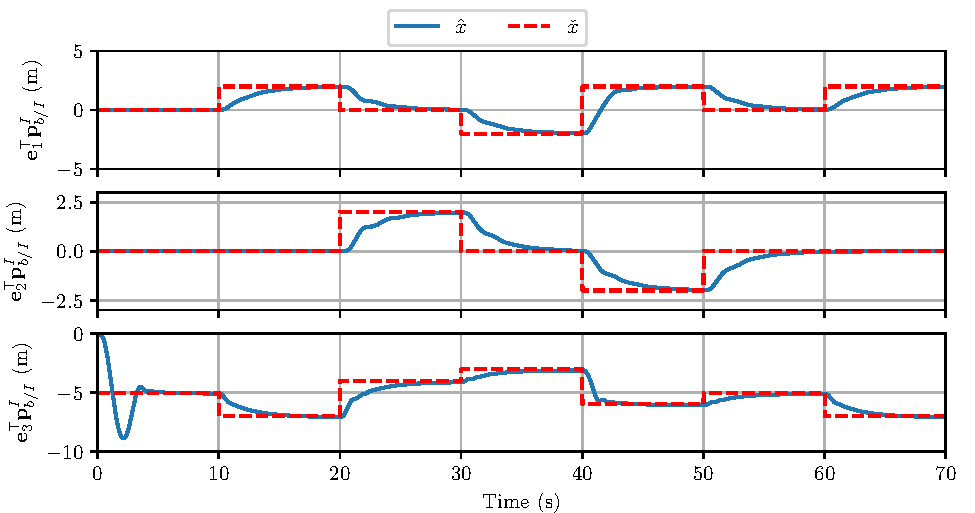
\includegraphics[width=0.6\textwidth]{figures/sim_wps_position}
  \caption[LQR Simulation Results Flying Waypoints]{Simulation results for the position of the multirotor UAV given step
  inputs to position. The red dotted line is the desired position and the blue
solid line is the estimated position.}
  \label{f:sim_wps}
\end{figure}

\begin{figure}
  \centering
  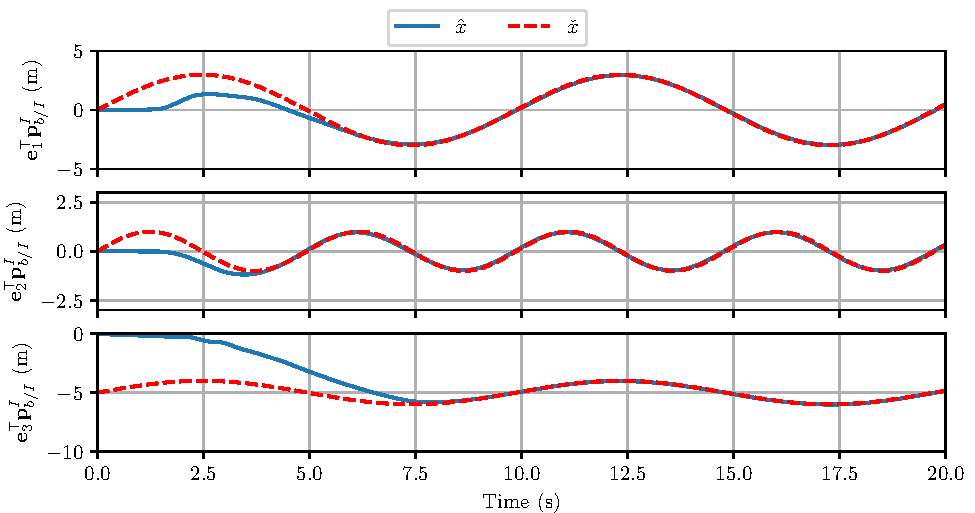
\includegraphics[width=0.6\textwidth]{figures/sim_fig8_position}
  \caption[LQR Simulation Results Flying a Trajectory]{Simulation results of a multirotor UAV tracking a figure eight
  trajectory. The red dotted line is the desired position and the blue solid
line is the estimated position.}
  \label{f:sim_fig8}
\end{figure}

Figs.~\ref{f:sim_wps} and~\ref{f:sim_fig8} show simulation results of the
controller following desired position step inputs (waypoints) and a figure-eight trajectory. The
multirotor begins the simulation at rest on the ground and converges to the
desired trajectory within a few seconds. Note that the figure-eight trajectory
tracking is near perfect even though the feed forward inputs computed
from~\eqref{eq:traj_p}{}--{}~\eqref{eq:traj_omega} do not account for the force due to drag and
the controller does not model thrust dynamics nor torque dynamics.

% !TEX root=../root.tex

\subsection{Hardware}

During the hardware experiments, the entire control algorithm was run at the
full streaming rate of the onboard IMU, which was set to 250 Hz. The computation
time of the algorithm was shown to have a mean of 274.6 $\upmu \mathrm{s}$ and a standard
deviation of 43.84 $\upmu \mathrm{s}$. This shows that the proposed LQR
formulation can run at full rate even on computationally constrained platforms.

\begin{figure}
  \centering
  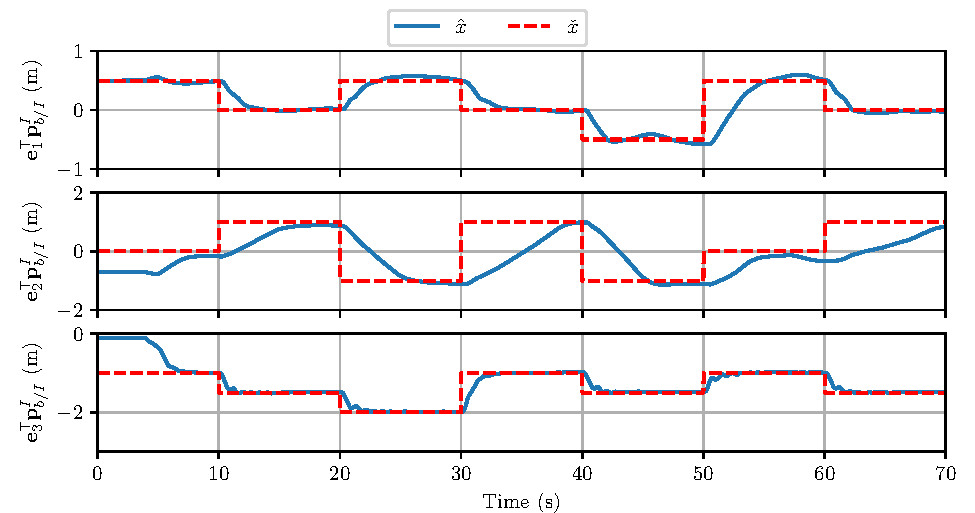
\includegraphics[width=0.4\textwidth]{figures/mocap_wps_position}
  \caption[LQR Hardware Results Flying Waypoints]{Hardware results for the position of the multirotor UAV given step
  inputs to position. The red dotted line is the desired position and the blue
solid line is the estimated position.}
  \label{f:hardware_wps}
\end{figure}

\begin{figure}
  \centering
  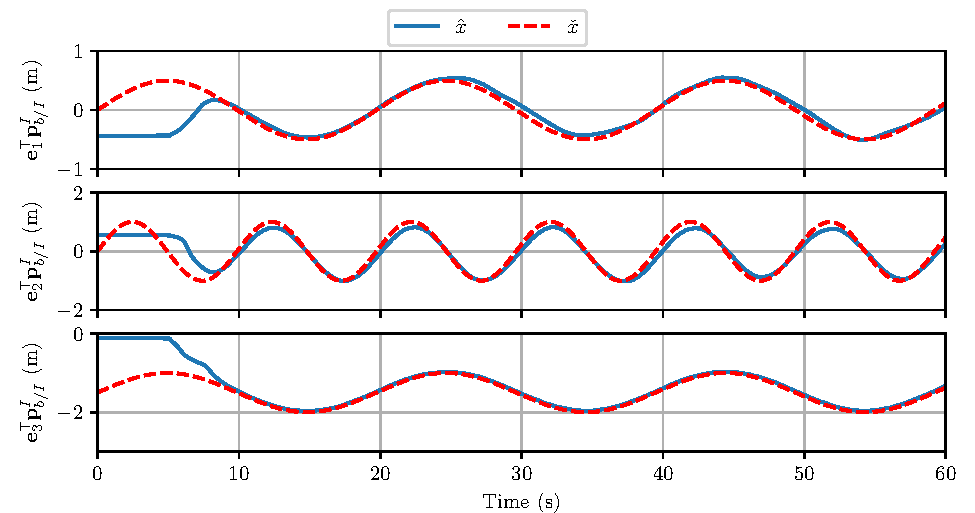
\includegraphics[width=0.4\textwidth]{figures/mocap_fig8_position}
  \caption[LQR Hardware Results Flying a Trajectory]{Hardware results of a multirotor UAV tracking a figure eight
  trajectory. The red dotted line is the desired position and the blue solid
line is the estimated position.}
  \label{f:hardware_fig8}
\end{figure}

\begin{figure}
  \centering
  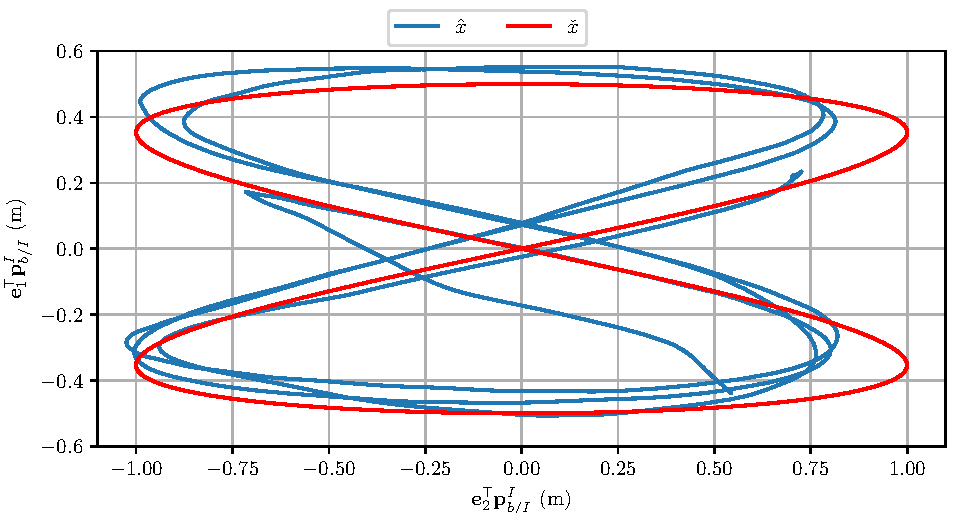
\includegraphics[width=0.4\textwidth]{figures/mocap_fig8_position_2d}
  \caption[Top Down View of LQR Hardware Trajectory]{Top down view of a multirotor UAV tracking a figure eight
  trajectory in hardware. The major deviation in position indicates the time
during take-off when the multirotor must get to the trajectory before following
it. The red solid line is the desired position and the blue solid line is the
estimated position.}
  \label{f:hardware_fig8_2d}
\end{figure}

Fig.~\ref{f:hardware_wps} shows the multirotor position along with the commanded
positions for a waypoint path. The clean step response with minimal overshoot is
notable considering we did not hand tune the LQR gains beyond an initial value
derived from Bryson's rule. Fig. \ref{f:hardware_fig8} shows how well the
multirotor is able to follow the figure-eight trajectory, and Fig.
\ref{f:hardware_fig8_2d} depicts the same flight plotted in two dimensions. The
major deviations visible in this plot depict the take-off and landing portions
of the flight.

% TX2
% 274.6 us mean, 43.84 us std

% Conclusion
\section{Conclusion} \label{sec:conclusion}
% !TEX root=../root.tex

%\subsection{Conclusion}

In this work we propose a novel LQR formulation derived from Lie theory. We
show that by using the error-state dynamics, we can properly compute control
using linear algebra techniques only on appropriate vector quantities. Our implementation is
efficient enough to relinearize the system and update the LQR gains in less than
one millisecond. Simulation and hardware experiments show the effectiveness and
simplicity of this control approach. 



% % What to do about this appendix
% % \appendix
% % \label{app:error_state_der}
% % % !TEX root=../root.tex

To derive the error-state dynamics of the multirotor UAV we first establish a few
identities and approximations. As it is convenient to work with rotation
matrices, we first write~\eqref{eq:q_des} in terms of rotation matrices. Since 
rotation matrices concatenate in an order opposite to quaterions, we have
\begin{equation}
  R_{I}^{b} = R\left(\exp_{\q}\left(\tilde{\vect{r}}_{I}^{b}\right)\right)
  \des{R}_{I}^{b}.
\end{equation}
With this, we can express the desired attitude as
\begin{equation}
  \des{R}_{I}^{b} =
  R\left(\exp_{\q}\left(\tilde{\vect{r}}_{I}^{b}\right)\right)^\transpose R_{I}^{b}.
\end{equation}
and when $\tilde{\vect{r}}_I^b$ is small, we employ~\eqref{eq:quaternion_exp_approx} to get
\begin{align}
  \des{R}_{I}^{b} &\approx R\left(
  \begin{bmatrix}1\\\frac{1}{2}\tilde{\vect{r}}_I^b\end{bmatrix}
\right)^\transpose R_{I}^{b} \\
  \phantom{\des{R}_{I}^{b}} &\approx R\left(
  \begin{bmatrix}1\\-\frac{1}{2}\tilde{\vect{r}}_I^b\end{bmatrix}
\right) R_{I}^{b}.
\end{align}
Now, we can substitute $R\left( \begin{bmatrix}1\\-\frac{1}{2}\tilde{\vect{r}}_I^b\end{bmatrix} \right)$ into eq.~\eqref{eq:R_from_q} to obtain
\begin{equation}
  \des{R}_{I}^{b} \approx \left( I + \skewmat{\tilde{\vect{r}}_I^b} \right)
  R_{I}^{b}.
\end{equation}
We also note that the transpose is given by
\begin{equation}
  \left(\des{R}_{I}^{b}\right)^\transpose =
  \left(R_{I}^{b}\right)^\transpose
  \left(R\left(\exp_{\q}\left(\tilde{\vect{r}}_{I}^{b}\right)\right)\right)
\end{equation}
and can be similarly approximated as
\begin{equation}
  \left(\des{R}_{I}^{b}\right)^\transpose \approx
  \left(R_{I}^{b}\right)^\transpose \left( I - \skewmat{\tilde{\vect{r}}_I^b}
  \right).
\end{equation}
We also employ the skew symmetric identity that
\begin{equation}
  \skewmat{\vect{a}} \vect{b} = -\skewmat{\vect{b}} \vect{a}.
\end{equation}

\subsection{Position}

Differentiating the error state for the position term given
by~\eqref{eq:pos_err} we get
%\begin{align}
%{\bf p}_{b/I}^{I} & =\left({\bf p}_{b/I}^{I}\right)_{\text{ref}}+{\bf \tilde{p}}_{b/I}^{I}\\
%\left({\bf p}_{b/I}^{I}\right)_{\text{ref}} & ={\bf p}_{b/I}^{I}-{\bf \tilde{p}}_{b/I}^{I}\\
%\tilde{{\bf p}}_{b/i}^{i} & ={\bf p}_{b/i}^{i}-\left({\bf p}_{b/i}^{i}\right)_{\text{ref}}.
%\end{align}
%Differentiating we get
\begin{equation}
  \dot{\tilde{\vect{p}}}_{b/I}^{I} = \dot{\vect{p}}_{b/I}^{I} -
    \dot{\des{\vect{p}}}_{b/I}^{I}.
\end{equation}
Substituting in the multirotor dynamics from~\eqref{eq:dynamics} and simplifying
we get
\begin{align}
  \dot{\tilde{\vect{p}}}_{b/I}^{I} &= \left(R_{I}^{b}\right)^\transpose
  \vect{v}_{b/I}^{b} - \left(\des{R}_{I}^{b}\right)^\transpose
  \des{\vect{v}}_{b/I}^{b} \\ 
  &= \left(R_{I}^{b}\right)^\transpose
  \vect{v}_{b/I}^{b} -
  \left(R\left(\exp_{\q}\left(\tilde{\vect{r}}_{I}^{b}\right)\right) R_{I}^{b}\right)^\transpose
  \des{\vect{v}}_{b/I}^{b} \\
  \begin{split}
  &= \left(R_{I}^{b}\right)^\transpose
  \vect{v}_{b/I}^{b}
  - \left(R_{I}^{b}\right)^\transpose
  \left(R\left(\exp_{\q}\left(\tilde{\vect{r}}_{I}^{b}\right)\right) \right)^\transpose
  \left(\vect{v}_{b/I}^{b} - \tilde{\vect{v}}_{b/I}^b\right) \\
  \end{split} \\
  \begin{split}
  &= \left(R_{I}^{b}\right)^\transpose
  \vect{v}_{b/I}^{b}
  - \left(R_{I}^{b}\right)^\transpose
  \left( I - \skewmat{\tilde{\vect{r}}_I^b}\right)
  \left(\vect{v}_{b/I}^{b} - \tilde{\vect{v}}_{b/I}^{b}\right).
  \end{split}
\end{align}
% \begin{align}
  % \dot{\tilde{\vect{p}}}_{b/I}^{I} &= \left(R_{I}^{b}\right)^\transpose
  % \vect{v}_{b/I}^{b} - \left(\des{R}_{I}^{b}\right)^\transpose
  % \des{\vect{v}}_{b/I}^{b} \\ 
  % &= \left(R_{I}^{b}\right)^\transpose
  % \vect{v}_{b/I}^{b} -
  % \left(R\left(\exp_{\q}\left(\tilde{\vect{r}}_{I}^{b}\right)\right) R_{I}^{b}\right)^\transpose
  % \des{\vect{v}}_{b/I}^{b} \\
  % \begin{split}
  % &= \left(R_{I}^{b}\right)^\transpose
  % \vect{v}_{b/I}^{b} \\
  % & \qquad - \left(R_{I}^{b}\right)^\transpose
  % \left(R\left(\exp_{\q}\left(\tilde{\vect{r}}_{I}^{b}\right)\right) \right)^\transpose
  % \left(\vect{v}_{b/I}^{b} - \tilde{\vect{v}}_{b/I}^b\right) \\
  % \end{split} \\
  % \begin{split}
  % &= \left(R_{I}^{b}\right)^\transpose
  % \vect{v}_{b/I}^{b} \\
  % & \qquad - \left(R_{I}^{b}\right)^\transpose
  % \left( I - \skewmat{\tilde{\vect{r}}_I^b}\right)
  % \left(\vect{v}_{b/I}^{b} - \tilde{\vect{v}}_{b/I}^{b}\right).
  % \end{split}
% \end{align}
By simplifying and neglecting higher-order terms, we get the final expression
\begin{equation}
  \dot{\tilde{\vect{p}}}_{b/I}^{I} = \left(R_{I}^{b}\right)^\transpose
  \tilde{\vect{v}}_{b/I}^{b} - \left(R_{I}^{b}\right)^\transpose
    \skewmat{\vect{v}_{b/I}^{b}} \tilde{\vect{r}}_I^b.
\end{equation}

\subsection{Velocity}

Differentiating the error state for the velocity term given
by~\eqref{eq:vel_err} we get
\begin{equation}
  \dot{\tilde{\vect{v}}}_{b/I}^{b} = \dot{\vect{v}}_{b/I}^{b} -
    \dot{\des{\vect{v}}}_{b/I}^{b}.
\end{equation}

Substituting in the multirotor dynamics from~\eqref{eq:dynamics} and simplifying
we get
\begin{align}
\begin{split}
  \dot{\tilde{\vect{v}}}_{b/I}^{b} ={}& \left(gR_I^b \vect{e}_3 -
    g\frac{s}{s_e}\vect{e}_3
    -\drag \left( I - \vect{e}_3 \vect{e}_3^\transpose \right) \vect{v}_{b/I}^b -
                  \skewmat{\vect{\omega}_{b/I}^b}\vect{v}_{b/I}^b\right) \\
    &- \left(g\des{R}_I^b \vect{e}_3 - g\frac{\des{s}}{s_e}\vect{e}_3
    - \drag \left( I - \vect{e}_3 \vect{e}_3^\transpose \right) \des{\vect{v}}_{b/I}^b -
    \skewmat{\des{\vect{\omega}}_{b/I}^b}\des{\vect{v}}_{b/I}^b\right) \\
\end{split} \\
\begin{split}
  \phantom{\dot{\tilde{\vect{v}}}_{b/I}^{b}}={}& \left(gR_I^b \vect{e}_3 -
  g\des{R}_I^b \vect{e}_3\right.) - \left(g\frac{s}{s_e}\vect{e}_3 -
      g\frac{\des{s}}{s_e}\vect{e}_3\right) \\
                                               &-\left(\drag \left( I - \vect{e}_3 \vect{e}_3^\transpose \right)
      \vect{v}_{b/I}^b
    - \drag \left( I - \vect{e}_3 \vect{e}_3^\transpose \right) \des{\vect{v}}_{b/I}^b
    \right) \\
    &- \left(\skewmat{\vect{\omega}_{b/I}^b}\vect{v}_{b/I}^b -
    \skewmat{\des{\vect{\omega}}_{b/I}^b} \des{\vect{v}}_{b/I}^b\right) \\
\end{split} \\
\begin{split}
  \phantom{\dot{\tilde{\vect{v}}}_{b/I}^{b}} \approx {}& \left(gR_I^b \vect{e}_3 -
    g\left( I + \skewmat{\tilde{\vect{r}}_I^b} \right) R_{I}^{b}
  \vect{e}_3\right) \\
    &-\left(g\frac{\tilde{s}}{s_e}\vect{e}_3\right)
    -\left(\drag \left( I - \vect{e}_3 \vect{e}_3^\transpose \right)
    \tilde{\vect{v}}_{b/I}^b\right) \\
    &- \left(\skewmat{\vect{\omega}_{b/I}^b}\vect{v}_{b/I}^b
    -\skewmat{\left(\vect{\omega}_{b/I}^{b} - \tilde{\vect{\omega}}_{b/I}^{b}\right)} 
  \left(\vect{v}_{b/I}^{b} - \tilde{\vect{v}}_{b/I}^{b}\right)\right) \\
\end{split} \\
\begin{split}
  \phantom{\dot{\tilde{\vect{v}}}_{b/I}^{b}} = {}& \left(-g
  \skewmat{\tilde{\vect{r}}_I^b} R_I^b \vect{e}_3\right)
    -\left(g\frac{\tilde{s}}{s_e}\vect{e}_3\right)
    -\left(\drag \left( I - \vect{e}_3 \vect{e}_3^\transpose \right)
    \tilde{\vect{v}}_{b/I}^b\right) \\
    &- \left(\skewmat{\vect{\omega}_{b/I}^b}\vect{v}_{b/I}^b
    -\skewmat{\left(\vect{\omega}_{b/I}^{b} - \tilde{\vect{\omega}}_{b/I}^{b}\right)} 
  \left(\vect{v}_{b/I}^{b} - \tilde{\vect{v}}_{b/I}^{b}\right)\right). \\
\end{split}
\end{align}
% \begin{align}
% \begin{split}
  % \dot{\tilde{\vect{v}}}_{b/I}^{b} ={}& \left(gR_I^b \vect{e}_3 -
    % g\frac{s}{s_e}\vect{e}_3\right. \\
    % &\left.-\drag \left( I - \vect{e}_3 \vect{e}_3^\transpose \right) \vect{v}_{b/I}^b -
                  % \skewmat{\vect{\omega}_{b/I}^b}\vect{v}_{b/I}^b\right) \\
    % &- \left(g\des{R}_I^b \vect{e}_3 - g\frac{\des{s}}{s_e}\vect{e}_3 \right. \\
    % &- \left.\drag \left( I - \vect{e}_3 \vect{e}_3^\transpose \right) \des{\vect{v}}_{b/I}^b -
    % \skewmat{\des{\vect{\omega}}_{b/I}^b}\des{\vect{v}}_{b/I}^b\right) \\
% \end{split} \\
% \begin{split}
  % \phantom{\dot{\tilde{\vect{v}}}_{b/I}^{b}}={}& \left(gR_I^b \vect{e}_3 -
  % g\des{R}_I^b \vect{e}_3\right.) - \left(g\frac{s}{s_e}\vect{e}_3 -
      % g\frac{\des{s}}{s_e}\vect{e}_3\right) \\
    % &-\left(\drag \left( I - \vect{e}_3 \vect{e}_3^\transpose \right)
      % \vect{v}_{b/I}^b\right. \\
    % &- \left.\drag \left( I - \vect{e}_3 \vect{e}_3^\transpose \right) \des{\vect{v}}_{b/I}^b
    % \right) \\
    % &- \left(\skewmat{\vect{\omega}_{b/I}^b}\vect{v}_{b/I}^b -
    % \skewmat{\des{\vect{\omega}}_{b/I}^b} \des{\vect{v}}_{b/I}^b\right) \\
% \end{split} \\
% \begin{split}
  % \phantom{\dot{\tilde{\vect{v}}}_{b/I}^{b}} \approx {}& \left(gR_I^b \vect{e}_3 -
    % g\left( I + \skewmat{\tilde{\vect{r}}_I^b} \right) R_{I}^{b}
  % \vect{e}_3\right) \\
    % &-\left(g\frac{\tilde{s}}{s_e}\vect{e}_3\right)
    % -\left(\drag \left( I - \vect{e}_3 \vect{e}_3^\transpose \right)
    % \tilde{\vect{v}}_{b/I}^b\right) \\
    % &- \left(\skewmat{\vect{\omega}_{b/I}^b}\vect{v}_{b/I}^b\right. \\
    % &-\left.\skewmat{\left(\vect{\omega}_{b/I}^{b} - \tilde{\vect{\omega}}_{b/I}^{b}\right)} 
  % \left(\vect{v}_{b/I}^{b} - \tilde{\vect{v}}_{b/I}^{b}\right)\right) \\
% \end{split} \\
% \begin{split}
  % \phantom{\dot{\tilde{\vect{v}}}_{b/I}^{b}} = {}& \left(-g
  % \skewmat{\tilde{\vect{r}}_I^b} R_I^b \vect{e}_3\right) \\
    % &-\left(g\frac{\tilde{s}}{s_e}\vect{e}_3\right)
    % -\left(\drag \left( I - \vect{e}_3 \vect{e}_3^\transpose \right)
    % \tilde{\vect{v}}_{b/I}^b\right) \\
    % &- \left(\skewmat{\vect{\omega}_{b/I}^b}\vect{v}_{b/I}^b\right. \\
    % &-\left.\skewmat{\left(\vect{\omega}_{b/I}^{b} - \tilde{\vect{\omega}}_{b/I}^{b}\right)} 
  % \left(\vect{v}_{b/I}^{b} - \tilde{\vect{v}}_{b/I}^{b}\right)\right). \\
% \end{split}
% \end{align}

By simplifying and neglecting higher-order terms, we get the final expression
\begin{equation}
  \begin{split}
  \dot{\tilde{\vect{v}}}_{b/I}^{b} = {}& g
  \skewmat{R_I^b \vect{e}_3} \tilde{\vect{r}}_I^b
    -g\frac{\tilde{s}}{s_e}\vect{e}_3
   -\drag \left( I - \vect{e}_3 \vect{e}_3^\transpose \right)
    \tilde{\vect{v}}_{b/I}^b \\
    &- \skewmat{\vect{\omega}_{b/I}^b} \tilde{\vect{v}}_{b/I}^b +
    \skewmat{\vect{v}_{b/I}^b} \tilde{\vect{\omega}}_{b/I}^b.
  \end{split}
\end{equation}
% \begin{equation}
  % \begin{split}
  % \dot{\tilde{\vect{v}}}_{b/I}^{b} = {}& g
  % \skewmat{R_I^b \vect{e}_3} \tilde{\vect{r}}_I^b
    % -g\frac{\tilde{s}}{s_e}\vect{e}_3 \\
    % &-\drag \left( I - \vect{e}_3 \vect{e}_3^\transpose \right)
    % \tilde{\vect{v}}_{b/I}^b \\
    % &- \skewmat{\vect{\omega}_{b/I}^b} \tilde{\vect{v}}_{b/I}^b +
    % \skewmat{\vect{v}_{b/I}^b} \tilde{\vect{\omega}}_{b/I}^b.
  % \end{split}
% \end{equation}

%\begin{multline}
  %\dot{\tilde{\vect{v}}}_{b/I}^{b} =\\
  %\left(gR_I^b \vect{e}_3 - g\frac{s}{s_e}\vect{e}_3 -
%\drag \left( I - \vect{e}_3 \vect{e}_3^\top \right) \vect{v}_{b/I}^b \\
%- \skewmat{\vect{\omega}_{b/I}^b}\vect{v}_{b/I}^b \right) \\
%- \left(gR_I^b \vect{e}_3 - g\frac{s}{s_e}\vect{e}_3 -
%\drag \left( I - \vect{e}_3 \vect{e}_3^\top \right) \vect{v}_{b/I}^b \\
%- \skewmat{\vect{\omega}_{b/I}^b}\vect{v}_{b/I}^b\right)
%\end{multline}

%\begin{align}
%\tilde{{\bf v}}_{b/i}^{b} & ={\bf v}_{b/i}^{b}-\left({\bf v}_{b/i}^{b}\right)_{\text{ref}}\\
 %& =\left(gR_{i}^{b}{\bf e}_{3}-F\frac{g}{F_{\text{hover}}}{\bf e}_{3}-M{\bf v}_{b/i}^{b}-\left({\bf \omega}_{b/i}^{b}\right)^{\wedge}{\bf v}_{b/i}^{b}\right)-\left(gR_{i}^{b}{\bf e}_{3}-F\frac{g}{F_{\text{hover}}}{\bf e}_{3}-M{\bf v}_{b/i}^{b}-\left({\bf \omega}_{b/i}^{b}\right)^{\wedge}{\bf v}_{b/i}^{b}\right)_{\text{ref}}\\
 %& =\left(gR_{i}^{b}{\bf e}_{3}-g\left(R_{i}^{b}\right)_{\text{ref}}{\bf e}_{3}\right)-\left(F\frac{g}{F_{\text{hover}}}{\bf e}_{3}-\left(F\right)_{\text{ref}}\frac{g}{F_{\text{hover}}}{\bf e}_{3}\right)-\left(M{\bf v}_{b/i}^{b}-M\left({\bf v}_{b/i}^{b}\right)_{\text{ref}}\right)-\left(\left({\bf \omega}_{b/i}^{b}\right)^{\wedge}{\bf v}_{b/i}^{b}-\left({\bf \omega}_{b/i}^{b}\right)_{\text{ref}}^{\wedge}\left({\bf v}_{b/i}^{b}\right)_{\text{ref}}\right)\\
 %& =g\left(R_{i}^{b}{\bf e}_{3}-R_{i}^{b}R\left(\exp\left(\tilde{{\bf q}}_{i}^{b}\right)\right){\bf e}_{3}\right)-\left(F\frac{g}{F_{\text{hover}}}{\bf e}_{3}-\left(F-\tilde{F}\right)\frac{g}{F_{\text{hover}}}{\bf e}_{3}\right)-\left(M{\bf v}_{b/i}^{b}-M\left({\bf v}_{b/i}^{b}-{\bf \tilde{v}}_{b/i}^{b}\right)\right)-\left(\left({\bf \omega}_{b/i}^{b}\right)^{\wedge}{\bf v}_{b/i}^{b}-\left({\bf \omega}_{b/i}^{b}-{\bf \tilde{\omega}}_{b/i}^{b}\right)^{\wedge}\left({\bf v}_{b/i}^{b}-{\bf \tilde{v}}_{b/i}^{b}\right)\right)\\
 %& \approx g\left(R_{i}^{b}{\bf e}_{3}-R_{i}^{b}\left(I-\left(\tilde{{\bf q}}_{I}^{b}\right)^{\wedge}\right){\bf e}_{3}\right)-\left(F\frac{g}{F_{\text{hover}}}{\bf e}_{3}-\left(F-\tilde{F}\right)\frac{g}{F_{\text{hover}}}{\bf e}_{3}\right)-\left(M{\bf v}_{b/i}^{b}-M\left({\bf v}_{b/i}^{b}-{\bf \tilde{v}}_{b/i}^{b}\right)\right)-\left(\left({\bf \omega}_{b/i}^{b}\right)^{\wedge}{\bf v}_{b/i}^{b}-\left({\bf \omega}_{b/i}^{b}-{\bf \tilde{\omega}}_{b/i}^{b}\right)^{\wedge}{\bf v}_{b/i}^{b}+\left({\bf \omega}_{b/i}^{b}-{\bf \tilde{\omega}}_{b/i}^{b}\right)^{\wedge}{\bf \tilde{v}}_{b/i}^{b}\right)\\
 %& =g\left(R_{i}^{b}{\bf e}_{3}-R_{i}^{b}{\bf e}_{3}+R_{i}^{b}\left(\tilde{{\bf q}}_{I}^{b}\right)^{\wedge}{\bf e}_{3}\right)-\left(\left(\tilde{F}\right)\frac{g}{F_{\text{hover}}}{\bf e}_{3}\right)-\left(M\left({\bf \tilde{v}}_{b/i}^{b}\right)\right)-\left(\left({\bf \omega}_{b/i}^{b}\right)^{\wedge}{\bf v}_{b/i}^{b}+\left({\bf v}_{b/i}^{b}\right)^{\wedge}\left({\bf \omega}_{b/i}^{b}-{\bf \tilde{\omega}}_{b/i}^{b}\right)-\left({\bf \tilde{v}}_{b/i}^{b}\right)^{\wedge}\left({\bf \omega}_{b/i}^{b}-{\bf \tilde{\omega}}_{b/i}^{b}\right)\right)\\
 %& =g\left(R_{i}^{b}\left(\tilde{{\bf q}}_{I}^{b}\right)^{\wedge}{\bf e}_{3}\right)-\left(\left(\tilde{F}\right)\frac{g}{F_{\text{hover}}}{\bf e}_{3}\right)-\left(M\left({\bf \tilde{v}}_{b/i}^{b}\right)\right)-\left(\left({\bf \omega}_{b/i}^{b}\right)^{\wedge}{\bf v}_{b/i}^{b}+\left({\bf v}_{b/i}^{b}\right)^{\wedge}{\bf \omega}_{b/i}^{b}-\left({\bf v}_{b/i}^{b}\right)^{\wedge}{\bf \tilde{\omega}}_{b/i}^{b}-\left({\bf \tilde{v}}_{b/i}^{b}\right)^{\wedge}{\bf \omega}_{b/i}^{b}+\left({\bf \tilde{v}}_{b/i}^{b}\right)^{\wedge}{\bf \tilde{\omega}}_{b/i}^{b}\right)\\
 %& =g\left(-R_{i}^{b}\left({\bf e}_{3}\right)^{\wedge}\left(\tilde{{\bf q}}_{I}^{b}\right)\right)-\left(\left(\tilde{F}\right)\frac{g}{F_{\text{hover}}}{\bf e}_{3}\right)-\left(M\left({\bf \tilde{v}}_{b/i}^{b}\right)\right)-\left(-\left({\bf v}_{b/i}^{b}\right)^{\wedge}{\bf \tilde{\omega}}_{b/i}^{b}+\left({\bf \omega}_{b/i}^{b}\right)^{\wedge}\left({\bf \tilde{v}}_{b/i}^{b}\right)\right)\\
 %& =-gR_{i}^{b}\left({\bf e}_{3}\right)^{\wedge}\left(\tilde{{\bf q}}_{I}^{b}\right)-\left(\tilde{F}\right)\frac{g}{F_{\text{hover}}}{\bf e}_{3}-M\left({\bf \tilde{v}}_{b/i}^{b}\right)+\left({\bf v}_{b/i}^{b}\right)^{\wedge}{\bf \tilde{\omega}}_{b/i}^{b}-\left({\bf \omega}_{b/i}^{b}\right)^{\wedge}\left({\bf \tilde{v}}_{b/i}^{b}\right)
%\end{align}


\subsection{Attitude}

To derive the error state dynamics corresponding to attitude, we start
with~\eqref{eq:rdot_diff}. From~\eqref{eq:r_def} we see that $\dot{\vect{r}}_I^b
= \vect{\omega}_{b/I}^b$. Substituting this defintion into~\eqref{eq:rdot_diff}
we get
\begin{equation}
\dot{\tilde{\vect{r}}}_I^b = \vect{\omega}_{b/I}^{b} -
R_I^b\left(\des{R}_I^b\right)^\transpose \des{\vect{\omega}}_{b/I}^{b}.
\end{equation}

We can simplify this expression and show that
\begin{align}
  \dot{\tilde{\vect{r}}}_I^b &= \vect{\omega}_{b/I}^{b} -
  R_I^b 
  \left(R_{I}^{b}\right)^\transpose
  \left(R\left(\exp_{\q}\left(\tilde{\vect{r}}_{I}^{b}\right)\right)\right)^\transpose
  \des{\vect{\omega}}_{b/I}^{b} \\
  &\approx \vect{\omega}_{b/I}^{b} -
  R_I^b \left(R_{I}^{b}\right)^\transpose \left( I - \skewmat{\tilde{\vect{r}}_I^b}
  \right) \des{\vect{\omega}}_{b/I}^{b} \\
  &= \vect{\omega}_{b/I}^{b} -
  \left( I - \skewmat{\tilde{\vect{r}}_I^b}
  \right) \left(\vect{\omega}_{b/I}^{b} - \tilde{\vect{\omega}}_{b/I}^{b}\right).
\end{align}
By simplifying and neglecting higher-order terms, we get the final expression
\begin{equation}
  \dot{\tilde{\vect{r}}}_I^b = \tilde{\vect{\omega}}_{b/I}^{b} -
  \skewmat{\vect{\omega}_{b/I}^{b} } \tilde{\vect{r}}_I^b.
\end{equation}


%Using rotation matrices
%\begin{align}
%\dot{R}_{i}^{b} & =R_{i}^{b}\left({\bf \omega}_{b/i}^{b}\right)^{\wedge}\\
%\left(R_{i}^{b}\right)_{\text{ref}} & =R_{I}^{b}R\left(\exp\left(\tilde{{\bf q}}_{I}^{b}\right)\right)
%\end{align}
%Following Sola, we can derive the attitude error state by looking
%at our two different, equivalent expresssions
%\begin{align}
%\dot{{\bf q}}_{i}^{b} & =\frac{1}{2}{\bf q}_{i}^{b}\otimes{\bf \omega}_{b/i}^{b}\\
%{\bf \dot{q}}_{i}^{b} & =\left(\dot{\left({\bf q}_{i}^{b}\right)_{\text{ref}}\otimes\tilde{{\bf q}}_{i}^{b}}\right)
%\end{align}
%With this, we can see that
%\begin{align}
%\left(\dot{\left({\bf q}_{i}^{b}\right)_{\text{ref}}\otimes\tilde{{\bf q}}_{i}^{b}}\right) & =\frac{1}{2}{\bf q}_{i}^{b}\otimes{\bf \omega}_{b/i}^{b}\\
%\left({\bf \dot{q}}_{i}^{b}\right)_{\text{ref}}\otimes\tilde{{\bf q}}_{i}^{b}+\left({\bf q}_{i}^{b}\right)_{\text{ref}}\otimes\dot{\tilde{{\bf q}}}_{i}^{b} & =\frac{1}{2}{\bf q}_{i}^{b}\otimes{\bf \omega}_{b/i}^{b}
%\end{align}
%OR ANOTHER WAY. Though the error state for the attitude term is given
%by 
%\begin{equation}
%\tilde{{\bf q}}_{I}^{b}={\bf q}_{I}^{b}\boxminus\left({\bf q}_{I}^{b}\right)_{\text{ref}}
%\end{equation}
%instead of differentiating through the $\boxminus$ operator, we instead
%use the derivative of attitude in its tanget space. Noting that the
%derivative of the reference attitude and the current attitude lie
%on different tangent spaces, we simply move one onto the other and
%perform regular subtraction because the tangent space is a vector
%space. We have
%\begin{align}
%\tilde{{\bf q}}_{i}^{b} & =\dot{{\bf q}}_{i}^{b}-R_{i}^{b}\left(R_{i}^{b}\right)_{\text{ref}}^{\top}\left({\bf \dot{q}}_{i}^{b}\right)_{\text{ref}}\\
 %& ={\bf \omega}_{b/i}^{b}-\left(R_{i}^{b}\right)\left(R_{i}^{b}\right)_{\text{ref}}^{\top}\left({\bf \omega}_{b/i}^{b}\right)_{\text{ref}}\\
 %& ={\bf \omega}_{b/i}^{b}-\left(R_{i}^{b}\right)\left(R\left(\exp\left(\tilde{{\bf q}}_{I}^{b}\right)\right)R_{I}^{b}\right)^{\top}\left({\bf \omega}_{b/i}^{b}+{\bf \tilde{\omega}}_{b/i}^{b}\right)\\
 %& \approx{\bf \omega}_{b/i}^{b}-\left(R_{i}^{b}\right)\left(R_{I}^{b}\right)^{\top}\left(I+\left(\tilde{{\bf q}}_{I}^{b}\right)^{\wedge}\right)\left({\bf \omega}_{b/i}^{b}+{\bf \tilde{\omega}}_{b/i}^{b}\right)\\
 %& ={\bf \omega}_{b/i}^{b}-\left(I+\left(\tilde{{\bf q}}_{I}^{b}\right)^{\wedge}\right)\left({\bf \omega}_{b/i}^{b}+{\bf \tilde{\omega}}_{b/i}^{b}\right)\\
 %& ={\bf \omega}_{b/i}^{b}-{\bf \omega}_{b/i}^{b}-{\bf \tilde{\omega}}_{b/i}^{b}-\left(\tilde{{\bf q}}_{I}^{b}\right)^{\wedge}{\bf \omega}_{b/i}^{b}-\left(\tilde{{\bf q}}_{I}^{b}\right)^{\wedge}{\bf \tilde{\omega}}_{b/i}^{b}\\
 %& \approx-{\bf \tilde{\omega}}_{b/i}^{b}-\left(\tilde{{\bf q}}_{I}^{b}\right)^{\wedge}{\bf \omega}_{b/i}^{b}\\
 %& =-{\bf \tilde{\omega}}_{b/i}^{b}+\left({\bf \omega}_{b/i}^{b}\right)^{\wedge}\left(\tilde{{\bf q}}_{I}^{b}\right)
%\end{align}



